% !TeX program = xelatex
% !TeX encoding = UTF-8
% Main editable manuscript. Figures are packaged in ./figures/.
% The original format reference is preserved in ../history/before_latex_migration/.
\documentclass[11pt,a4paper]{article}
\usepackage{fontspec}
\usepackage{amsmath,amssymb}
\usepackage{tikz}
\usetikzlibrary{arrows.meta,positioning}
\usepackage{geometry}
\geometry{a4paper,margin=1in}
\usepackage{graphicx,booktabs,tabularx,array}
\usepackage{caption}
\usepackage[section]{placeins}
\usepackage{flafter}
\usepackage{float,needspace}
\usepackage[nocompress]{cite}
\usepackage{etoolbox}
\renewcommand{\citepunct}{],\,[}
\usepackage[unicode,hidelinks]{hyperref}
\hypersetup{pdftitle={Passive localization of spectrally overlapping strong and weak sources from short observations},pdfsubject={Academic research report}}
\numberwithin{equation}{section}
\numberwithin{figure}{section}
\numberwithin{table}{section}
\renewcommand{\figurename}{Figure}
\renewcommand{\tablename}{Table}
\renewcommand{\contentsname}{Contents}
\captionsetup{justification=centering,singlelinecheck=false,labelsep=quad,font=small,labelfont=bf}
\captionsetup[table]{position=top,skip=6pt}
\newcolumntype{Y}[1]{>{\hsize=#1\hsize\linewidth=\hsize\raggedright\arraybackslash}X}
\patchcmd{\thebibliography}{\section*{\refname}}{}{}{}
\setlength{\intextsep}{8pt plus 2pt minus 2pt}
\setlength{\textfloatsep}{10pt plus 2pt minus 2pt}
\setlength{\floatsep}{8pt plus 2pt minus 2pt}
\setcounter{tocdepth}{1}
\setcounter{secnumdepth}{3}
\setlength{\parindent}{1.5em}
\setlength{\parskip}{.15em}
\setlength{\emergencystretch}{2em}
\linespread{1.12}
\renewcommand{\topfraction}{.9}
\renewcommand{\bottomfraction}{.8}
\renewcommand{\textfraction}{.08}
\renewcommand{\floatpagefraction}{.75}
\setcounter{topnumber}{3}        
\setcounter{totalnumber}{5}
\raggedbottom
\clubpenalty=10000
\widowpenalty=10000
\displaywidowpenalty=10000
\title{\bfseries Passive localization of spectrally overlapping strong and weak sources from short observations}
\author{}
\date{}
\makeatletter
\renewcommand{\@maketitle}{\begin{center}{\LARGE\@title\par}\end{center}\vspace{1em}}
\makeatother

\begin{document}
\maketitle
% Source block 2
\section*{Abstract}

% Source block 3
Spectral overlap and unequal received powers complicate delay extraction and association across receivers in passive multisource localization. This report considers four synchronized single-antenna receivers and two sources under line-of-sight propagation, with unknown complex gains shared across frequencies. Eliminating the unknown waveforms gives a joint least-squares objective. A largest-eigenvalue spatial spectrum is derived from single-source LS and extended to alternating updates on multisource residuals. Its relationship to projected conditional spectra, MUSIC-type DPD, and DPD-HR is established. Local identifiability and curvature are discussed with both waveform and gain nuisance parameters included. A planned comparison holds weak-source power and noise fixed while increasing the received-power difference from 0 to 15 dB, and evaluates localization accuracy, success rates, error distributions, and total processing time for both sources. Results with unknown gains are pending. The appendices retain derivations and experiments with known relative gains as evidence about candidate omission and search cost under that assumption, not as performance evidence for the new model.

% Source block 7
\section{Introduction}\label{sec:1}

% Source block 8
\subsection{Application context and overlapping sources}\label{sec:1.1}

% Source block 9
In distributed spectrum monitoring and localization of noncooperative emitters, the transmitted waveforms and transmission times are usually unavailable. Positions must therefore be inferred from observations at multiple receivers. Several emitters may occupy the same reception band, so each record contains a mixture of sources. Differences in transmit power and propagation distance produce unequal received powers. Here, spectral overlap means overlap between frequency supports; it does not refer to aliasing caused by undersampling.

% Source block 10
The setting of interest is a weak source that can be localized in isolation but is often mislocalized when a strong source is present. Strong and weak are defined by received power averaged across the receiver network; the same source need not be stronger at every receiver. With short observations, fluctuations in sample correlations and cross terms between sources also affect estimation. Both sources must be localized within a limited processing time, so strong-source accuracy alone is insufficient to assess performance.

% Source block 11
\subsection{Difficulties in two-step localization and the DPD approach}\label{sec:1.2}

% Source block 12
Conventional two-step localization first estimates time differences of arrival (TDOAs) from receiver pairs, then solves for position using the resulting geometric constraints. Generalized cross-correlation provides a basic framework for delay estimation\cite{ref01}. The hyperbolic estimator of Chan and Ho and subsequent bias analysis address the position solution given delay measurements\cite{ref02,ref03}.

% Source block 13
For a mixture of strong and weak sources, cross-correlation between receivers contains shifted autocorrelation terms from each source, finite-sample cross terms, and noise. Strong-source terms may mask the weak-source peak. Even if several peaks are retained, the delays from different receiver pairs must still be associated with the same source. Selecting the largest peak independently for each pair can produce delays that are inconsistent with any single position. These difficulties arise in measurement extraction and association, before the geometric position solution.

% Source block 14
DPD constructs an estimation objective directly from the received signals and the propagation responses of candidate positions. The observations thus constrain position jointly across receivers. Weiss and Amar discuss the distinction between direct and two-step localization, including the association problem for multiple sources\cite{ref04}. DPD is used here to avoid committing prematurely to a single delay peak at the front end. Coupling between sources and the search over a multimodal objective remain.

% Source block 15
\subsection{Related work and research question}\label{sec:1.3}
Chen et al. formulate maximum-likelihood localization from wideband observations and eliminate unknown waveforms in joint estimation\cite{ref05}. A single-source model with unknown gains leads to a largest-eigenvalue score; multisource estimation requires a distinction between joint fitting and pointwise scanning. The multisource DPD of Weiss and Amar uses signal subspaces\cite{ref04}, whereas DPD-HR combines direct localization with a minimum-variance criterion and inverse covariance matrices\cite{ref06}. Their statistical observation requirements must be consistent with short records.

The more recent DPD-PDL estimates off-grid position offsets and unknown complex attenuation jointly in sparse direct localization with single-antenna receivers\cite{ref13}. Other multisource ML methods use CSI obtained from a common known reference signal\cite{ref14}, which differs from a mixture of unknown independent waveforms. Method selection therefore depends on observations, unknown parameters, and computational cost, not publication date alone.

Projection, candidate retention, and cyclic refinement also appear in multisource estimation. Round-robin localization uses projection and position revisits\cite{ref07}; NOMP combines component detection with continuous refinement\cite{ref08}; SRP and group-sparse methods retain multiple direction candidates\cite{ref09}. Their search ideas are relevant, but results from the original acoustic, sinusoidal, or array models do not transfer directly to the present setting.

This report first establishes the relationships between the observation model, spatial spectra, and joint objective, then specifies a comparison of representative methods as the received-power ratio changes. Weak-source power is calibrated independently and fixed; only the other source becomes stronger. The need for mechanism analysis or a new solver will be judged from those comparisons. Existing derivations and results with known relative gains are retained in Appendices~\ref{sec:2}--\ref{sec:4} and interpreted separately from the unknown-gain model.

% Main sections for the unknown-complex-gain model. Edit directly.
\section{Problem formulation and localization methods}\label{sec:ug-model}
\subsection{Geometry, propagation, and unknown parameters}\label{sec:ug-assumptions}
Consider $L$ synchronized single-antenna receivers at known positions and $K$ stationary emitters. The primary scenario uses $L=4$ and $K=2$. Receiver and source positions are $\mathbf r_\ell\in\mathbb R^2$ and $\mathbf p_k\in\Omega$, where $\Omega=[-1000,1000]^2\ \mathrm{m}^2$. The propagation distance is $d_{\ell k}=\|\mathbf p_k-\mathbf r_\ell\|$, and the delay is $\tau_{\ell k}=d_{\ell k}/c$, with known propagation speed $c$. The source count, receiver positions, and synchronization are known; source waveforms, transmit powers, and complex gains across receivers are unknown. The sources are generated independently, but their cross terms need not vanish in a finite record.

The simulator uses free-space line-of-sight propagation. For fixed carrier frequency and antenna characteristics, received field amplitude is proportional to $1/d_{\ell k}$ and power to $1/d_{\ell k}^2$. A common scale can be absorbed into the waveform, and carrier propagation phase into the complex gain. The estimator treats the gains across receivers as unknown instead of imposing relative amplitudes determined by distance. The time-domain model is
\begin{equation}\label{eq:ug-time}
x_\ell[n]=\sum_{k=1}^K\beta_{\ell k}v_k(nT_s-\tau_{\ell k})+w_\ell[n],
\quad w_\ell[n]\sim\mathcal{CN}(0,\sigma_t^2).
\end{equation}
Here $T_s=1/F_s$ and $n=0,\ldots,N-1$; receiver noises are independent and have equal variance. Each complex gain is constant over the observation and the frequency band used. Let $\mathbf g_k=[\beta_{1k},\ldots,\beta_{Lk}]^T$ and $\mathbf b_k=\mathbf g_k/\|\mathbf g_k\|$. Absorb its norm into the source waveform and fix the phase of a nonzero reference component:
\begin{equation}\label{eq:ug-gauge}
\|\mathbf b_k\|=1,\qquad
\operatorname{Im}b_{\ell_0 k}=0,\quad \operatorname{Re}b_{\ell_0 k}>0.
\end{equation}
If the reference component is zero, use a nonzero component for the local parameterization. These constraints remove the scale and common-phase ambiguities between gain and waveform. They do not normalize the energy of the received observations.

With a DFT divided by $N$, the noise variance is $\sigma_f^2=\sigma_t^2/N$. Using a frequency-domain approximation that neglects observation-window edge effects\cite{ref04,ref05}, and retaining signed baseband frequencies $f_m$, gives
\begin{equation}\label{eq:ug-model}
\begin{aligned}
\mathbf x_m&=\sum_{k=1}^K\mathbf D_m(\mathbf p_k)\mathbf b_k s_{k,m}+\mathbf n_m
=\mathbf A_m(\theta,\mathbf B)\mathbf s_m+\mathbf n_m,\\
\mathbf D_m(\mathbf p)&=\operatorname{diag}_{\ell=1}^L
\{e^{-j2\pi f_m\tau_\ell(\mathbf p)}\},\qquad
\mathbf n_m\sim\mathcal{CN}(\mathbf0,\sigma_f^2\mathbf I_L).
\end{aligned}
\end{equation}
Here $\theta=[\mathbf p_1^T,\ldots,\mathbf p_K^T]^T$, $\mathbf B=[\mathbf b_1,\ldots,\mathbf b_K]$, and $\mathbf A_m=[\mathbf D_m(\mathbf p_1)\mathbf b_1,\ldots,\mathbf D_m(\mathbf p_K)\mathbf b_K]$. Positions and gains are shared across frequencies, whereas $\mathbf s_m$ is unknown at each frequency. Arbitrary, independently varying gains at every receiver and frequency could absorb the delay phases and remove the corresponding localization constraints.

\begin{table}[!htbp]
\centering\caption{Main notation for the unknown-gain model.}\label{tab:ug-symbols}
\small\renewcommand{\arraystretch}{1.15}
\begin{tabularx}{\linewidth}{Y{.8}Y{1.5}Y{.7}}
\toprule Symbol & Meaning & Dimension or unit\\\midrule
$\theta,\mathbf B$ & Position vector and normalized unknown complex gains & $2K\times1$, $L\times K$\\
$\mathbf x_m,\mathbf s_m$ & Receiver observations and source coefficients & $L\times1$, $K\times1$\\
$\mathbf D_m,\mathbf A_m$ & Delay-phase matrix and multisource response & $L\times L$, $L\times K$\\
$\mathbf P_m^\perp$ & Orthogonal complement of the response column space & $L\times L$\\
$\mathbf R_k(\mathbf p)$ & Correlation of delay-compensated residuals for source $k$ & $L\times L$\\
$\gamma,\Delta P$ & Weak-to-strong received-power ratio and power difference & Dimensionless, dB\\
\bottomrule\end{tabularx}
\end{table}
Superscripts $H$ and $\dagger$ denote the conjugate transpose and Moore--Penrose pseudoinverse. In the main text, $\mathbf D_m$ denotes the delay-phase matrix. Appendix~\ref{sec:2} uses the same letter locally for derivatives of the mean.

\subsection{Waveform elimination and joint least squares}\label{sec:ug-ls}
Under~\eqref{eq:ug-model}, the negative log-likelihood, apart from a constant, is the total residual divided by $\sigma_f^2$. Define
\begin{equation}\label{eq:ug-full-ls}
\mathcal L(\theta,\mathbf B,\{\mathbf s_m\})
=\sum_m\|\mathbf x_m-\mathbf A_m\mathbf s_m\|^2.
\end{equation}
For fixed positions and gains, the waveform coefficients form a linear least-squares (LS) subproblem. Substituting its minimum-norm solution gives
\begin{equation}\label{eq:ug-profile}
\begin{aligned}
\widehat{\mathbf s}_m&=\mathbf A_m^\dagger\mathbf x_m,\qquad
\mathbf P_m^\perp=\mathbf I_L-\mathbf A_m\mathbf A_m^\dagger,\\
J(\theta,\mathbf B)&=\min_{\{\mathbf s_m\}}\mathcal L
=\sum_m\|\mathbf P_m^\perp\mathbf x_m\|^2,\\
(\widehat\theta,\widehat{\mathbf B})&\in
\arg\min_{\theta\in\Omega^K,\,\mathbf B\in\mathcal G}
J(\theta,\mathbf B).
\end{aligned}
\end{equation}
The set $\mathcal G$ imposes~\eqref{eq:ug-gauge}. Waveform elimination does not eliminate the gains. Each complex gain vector has $2L-2$ real degrees of freedom after removing its two ambiguities. With four receivers and two sources, there are four position parameters and twelve real gain degrees of freedom. A position-only profile objective can be defined formally as
\begin{equation}\label{eq:ug-position-profile}
J_{\mathrm{pos}}(\theta)=\min_{\mathbf B}J(\theta,\mathbf B).
\end{equation}
An inner solver that finds only a local gain solution does not, in general, evaluate the exact minimum in~\eqref{eq:ug-position-profile}. Comparisons of general-purpose optimizers must use the same objective, gain constraints, and inner-solver convention, including the time spent estimating gains.

\subsection{From single-source LS to a largest-eigenvalue spectrum}\label{sec:ug-single}
Set $K=1$. Compensate the delays at candidate position $\mathbf p$ by defining $\mathbf y_m(\mathbf p)=\mathbf D_m^H(\mathbf p)\mathbf x_m$. Since $\mathbf D_m$ is unitary and $\|\mathbf b\|=1$,
\begin{equation}\label{eq:ug-single-elimination}
\begin{aligned}
\min_{\{s_m\}}\sum_m\|\mathbf y_m-\mathbf b s_m\|^2
&=E_x-\mathbf b^H\mathbf R(\mathbf p)\mathbf b,\\
\widehat s_m&=\mathbf b^H\mathbf y_m,\quad
\mathbf R(\mathbf p)=\sum_m\mathbf y_m\mathbf y_m^H,\quad
E_x=\sum_m\|\mathbf x_m\|^2.
\end{aligned}
\end{equation}
The extremum of the Rayleigh quotient gives
\begin{equation}\label{eq:ug-single-eigen}
\max_{\|\mathbf b\|=1}\mathbf b^H\mathbf R(\mathbf p)\mathbf b
=\lambda_{\max}(\mathbf R(\mathbf p)),\qquad
\widehat{\mathbf p}\in\arg\max_{\mathbf p\in\Omega}
\lambda_{\max}(\mathbf R(\mathbf p)).
\end{equation}
The optimal gain direction is a unit eigenvector associated with the largest eigenvalue, with its common phase adjusted according to~\eqref{eq:ug-gauge}. This derivation connects LS, waveform elimination, and largest-eigenvalue scanning\cite{ref05,ref06}. Applying the same score to a mixture and selecting several peaks uses a pointwise single-source criterion; it is generally not the joint multisource ML estimator.

\subsection{Eigenvalue updates on multisource residuals}\label{sec:ug-block}
When updating source $k$, hold the positions, gains, and waveforms of the other sources fixed and subtract their fitted signals:
\begin{equation}\label{eq:ug-residual}
\mathbf e_{k,m}=\mathbf x_m-
\sum_{q\ne k}\mathbf D_m(\mathbf p_q)\mathbf b_qs_{q,m},\qquad
\mathbf y_{k,m}(\mathbf p)=\mathbf D_m^H(\mathbf p)\mathbf e_{k,m}.
\end{equation}
Applying the preceding elimination to this residual yields
\begin{equation}\label{eq:ug-block-eigen}
\begin{aligned}
\min_{\|\mathbf b_k\|=1,\{s_{k,m}\}}
\sum_m\|\mathbf e_{k,m}-\mathbf D_m(\mathbf p)\mathbf b_ks_{k,m}\|^2
&=E_k-\lambda_{\max}(\mathbf R_k(\mathbf p)),\\
E_k=\sum_m\|\mathbf e_{k,m}\|^2,\qquad
\mathbf R_k(\mathbf p)&=\sum_m\mathbf y_{k,m}\mathbf y_{k,m}^H.
\end{aligned}
\end{equation}
After scanning or continuously optimizing $\mathbf p$, update $\mathbf b_k$ using the principal eigenvector and set $s_{k,m}=\mathbf b_k^H\mathbf y_{k,m}$. Update the sources in turn; all waveforms may then be jointly refitted using~\eqref{eq:ug-profile}. Retaining the previous solution and accepting only updates that do not increase~\eqref{eq:ug-full-ls} ensures a nonincreasing residual. It does not ensure a global optimum. Finite position searches, errors in the initial residual, and stopping criteria can all affect the estimate.

\subsection{Projected conditional spectra and MUSIC-type DPD}\label{sec:ug-spectra}
Residual subtraction fixes the other waveforms, whereas orthogonal projection allows them to be refitted. For fixed positions and gains of the other sources, let $\mathbf A_{-k,m}$ contain their responses and $\mathbf P_{-k,m}^\perp=\mathbf I-\mathbf A_{-k,m}\mathbf A_{-k,m}^\dagger$. The reduction in residual obtained by adding a response is
\begin{equation}\label{eq:ug-projection}
Q(\mathbf p,\mathbf b)=\sum_m
\frac{|\mathbf b^H\mathbf D_m^H(\mathbf p)\mathbf P_{-k,m}^\perp\mathbf x_m|^2}
{\mathbf b^H\mathbf D_m^H(\mathbf p)\mathbf P_{-k,m}^\perp\mathbf D_m(\mathbf p)\mathbf b}.
\end{equation}
A zero projected response contributes zero. For fixed $\mathbf b$, this is the exact improvement in joint LS. Optimizing the frequency-shared $\mathbf b$ generally involves a sum of Rayleigh quotients with different denominators and does not reduce to one ordinary eigendecomposition. The conditional spectrum in Appendix~\ref{sec:2} follows this projection route with known relative gains.

MUSIC-type DPD uses orthogonality between signal and noise subspaces\cite{ref04}. Suppose the same observation record provides $J_s$ usable statistical segments, with frequency-domain observation $\mathbf x_{m,j}$ in segment $j$. Form
\begin{equation}\label{eq:ug-covariance}
\widehat{\mathbf R}_{x,m}=\frac1{J_s}\sum_{j=1}^{J_s}\mathbf x_{m,j}\mathbf x_{m,j}^H
=\mathbf U_{s,m}\Lambda_{s,m}\mathbf U_{s,m}^H+
\mathbf U_{n,m}\Lambda_{n,m}\mathbf U_{n,m}^H.
\end{equation}
In the population model, with equal noise variances, a full-rank source covariance, and correctly separated subspaces, a true response satisfies
\[\mathbf U_{n,m}^H\mathbf D_m(\mathbf p_k)\mathbf b_k=0.\]
For fixed weights $w_m\geq0$ with $\sum_mw_m=1$, eliminating the unit-norm unknown gain gives
\begin{equation}\label{eq:ug-music}
\begin{aligned}
\mathbf C(\mathbf p)&=\sum_mw_m\mathbf D_m^H(\mathbf p)
\mathbf U_{n,m}\mathbf U_{n,m}^H\mathbf D_m(\mathbf p),\\
P_{\mathrm{MUSIC}}(\mathbf p)&=\left[
\min_{\|\mathbf b\|=1}\mathbf b^H\mathbf C(\mathbf p)\mathbf b\right]^{-1}
=\frac1{\lambda_{\min}(\mathbf C(\mathbf p))}.
\end{aligned}
\end{equation}
Since the signal and noise projectors sum to the identity, the denominator also equals $1-\lambda_{\max}(\sum_mw_m\mathbf D_m^H\mathbf U_{s,m}\mathbf U_{s,m}^H\mathbf D_m)$. This matrix contains subspace projectors, unlike the raw correlation matrix in~\eqref{eq:ug-single-eigen}. With one antenna per receiver and only one frequency, the unitary similarity transform preserves the eigenvalues and cannot localize a source through this spectrum. Shared gains and constraints across multiple frequencies are therefore essential.

DPD-HR uses inverse covariance matrices to form another score. Its single-antenna structure is\cite{ref06}
\begin{equation}\label{eq:ug-hr}
P_{\mathrm{HR}}(\mathbf p)=
\frac1{\lambda_{\min}\!\left(\sum_mw_m\mathbf D_m^H(\mathbf p)
\widehat{\mathbf R}_{x,m}^{-1}\mathbf D_m(\mathbf p)\right)}.
\end{equation}
Segmentation must support both the delay-model approximation and covariance estimation. Loading or regularization for singular matrices must be stated. Snapshots from other Monte Carlo trials cannot be pooled, and the total observation duration cannot be increased for a comparison. Equations~\eqref{eq:ug-music} and~\eqref{eq:ug-hr} explain the method relationships; their implementation and performance with the present short records remain to be checked.

\subsection{Compared methods and the complete estimation flow}\label{sec:ug-methods}
\begin{table}[!htbp]
\centering\caption{Planned comparisons with unknown gains.}\label{tab:ug-methods}
\small\renewcommand{\arraystretch}{1.15}
\begin{tabularx}{\linewidth}{Y{.8}Y{1.25}Y{.95}}
\toprule Method & Estimation criterion & Settings to fix\\\midrule
Single-source eigenvalue scan with multiple peaks & Equation~\eqref{eq:ug-single-eigen} & Full-region candidates, peak selection, refinement\\
MUSIC-type DPD & Equation~\eqref{eq:ug-music} & Segments, signal-subspace rank, frequency weights\\
DPD-HR/MVDR & Equation~\eqref{eq:ug-hr} & Segments, covariance estimation, regularization\\
Alternating joint LS & Equations~\eqref{eq:ug-full-ls} and~\eqref{eq:ug-block-eigen} & Initialization, source searches, joint waveform updates\\
Multistart local optimization, differential evolution, GA & The same objective in~\eqref{eq:ug-profile} & Identical gain constraints and total processing budgets\\
DPD-PDL & Sparse Bayesian estimation with a parametric dictionary & Full-region dictionary, complex gains, off-grid updates\\
Unknown-gain versions of A--D & Supplementary search comparisons for~\eqref{eq:ug-profile} & Adaptation and new evaluation; no reuse of old scores\\
\bottomrule\end{tabularx}
\end{table}
Table~\ref{tab:ug-methods} separates estimation criteria from solvers. A genetic algorithm (GA), differential evolution, and multistart local optimization are solvers, not additional observation models. Solvers for the same joint objective must receive the same information and constraints.

DPD-PDL incorporates off-grid position offsets and unknown complex attenuation into a parametric dictionary and updates them within sparse Bayesian learning\cite{ref13}. Its observations are close to the single-antenna multireceiver model, making it a priority for qualification. Initialization, the cost of a full-region dictionary, and the complex-valued update equations still require inspection. Multisource ML using CSI obtained from a common known reference signal\cite{ref14} has different observation information. Its path gains may remain unknown; CSI should not be equated with known gains.

\begin{figure}[!htbp]\centering
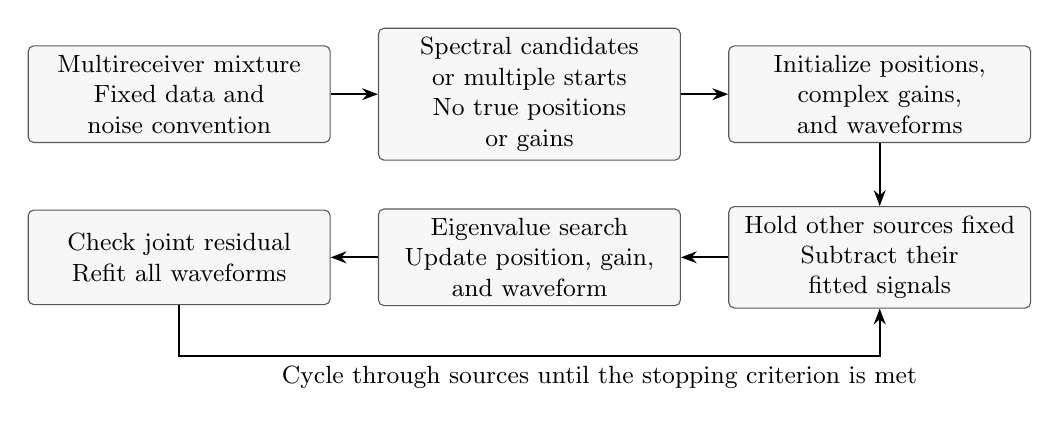
\begin{tikzpicture}[node distance=8mm and 6mm,
box/.style={draw=black!65,fill=black!3,rounded corners=2pt,text width=3.6cm,minimum height=12mm,align=center,font=\small},
arr/.style={-{Stealth[length=2mm]},thick}]
\node[box] (iq) {Multireceiver mixture\\Fixed data and noise convention};
\node[box,right=of iq] (init) {Spectral candidates\\or multiple starts\\No true positions\\or gains};
\node[box,right=of init] (state) {Initialize positions, complex gains, and waveforms};
\node[box,below=of state] (res) {Hold other sources fixed\\Subtract their fitted signals};
\node[box,left=of res] (update) {Eigenvalue search\\Update position, gain,\\and waveform};
\node[box,left=of update] (accept) {Check joint residual\\Refit all waveforms};
\draw[arr] (iq)--(init);\draw[arr] (init)--(state);\draw[arr] (state)--(res);
\draw[arr] (res)--(update);\draw[arr] (update)--(accept);
\draw[arr] (accept.south)--++(0,-.65)-|node[pos=.3,below,font=\small]{Cycle through sources until the stopping criterion is met} (res.south);
\end{tikzpicture}
\caption{An alternating joint-LS solver with unknown gains.}\label{fig:ug-flow}
\end{figure}
Figure~\ref{fig:ug-flow} connects spectral candidates to joint fitting. A spatial spectrum can also produce a direct multiple-peak estimate. General-purpose optimizers may update positions and gains jointly without using these source-by-source steps. Initialization effects require comparisons with a fixed solver and budget; they cannot be inferred from differences between complete algorithms.

The unit-norm gain constraints and division by snapshot count in the classical derivations\cite{ref04,ref06} differ from scaling each receiver by the RMS of its mixed observation. The main comparison uses raw observations without this energy equalization. A receiver scaling matrix $\mathbf W=\operatorname{diag}(w_1,\ldots,w_L)$ changes the noise covariance to $\sigma_f^2\mathbf W\mathbf W^H$; unweighted LS on the scaled data therefore changes the criterion. Weights obtained from mixed observations also vary with strong-source power, so the RMS version is evaluated separately. Dividing a displayed spectrum by its maximum or expressing it in relative dB does not change the estimator.

\subsection{Identifiability, local curvature, and nonconvex optimization}\label{sec:ug-information}
The joint objective after waveform elimination is generally nonconvex. Convexity of the linear LS subproblem with a fixed response does not imply convexity of position optimization through delay phases. Nor does convexity of the largest eigenvalue as a function of a matrix imply convexity of the position search.

In a smooth local parameterization with the ambiguities fixed, let $\eta$ collect real nuisance parameters for waveforms and gains, and let $\boldsymbol{\mu}$ be the stacked observation mean. The information blocks and effective position information are
\begin{equation}\label{eq:ug-fim}
\begin{aligned}
\mathbf I_{ab}&=\frac{2}{\sigma_f^2}\operatorname{Re}
\left\{\left(\frac{\partial\boldsymbol{\mu}}{\partial a}\right)^H
\frac{\partial\boldsymbol{\mu}}{\partial b}\right\},\quad a,b\in\{\theta,\eta\},\\
\mathbf I_{\theta}^{\mathrm{eff}}&=\mathbf I_{\theta\theta}
-\mathbf I_{\theta\eta}\mathbf I_{\eta\eta}^{-1}\mathbf I_{\eta\theta}.
\end{aligned}
\end{equation}
The inverse-block expression in~\eqref{eq:ug-fim} requires local identifiability of the relevant parameters. Singular cases require treatment of unidentifiable directions before asserting a finite position CRB\cite{ref10}. Position derivatives at fixed unknown gains differentiate the delay phases, not the simulator's $1/d$ amplitude law. The old information matrix, which eliminates only waveforms, cannot replace this expression.

For local real parameters $z$, smooth complex residual $\boldsymbol{\rho}(z)$, and $\mathbf G=\partial\boldsymbol{\rho}/\partial z$,
\begin{equation}\label{eq:ug-hessian}
\nabla^2\|\boldsymbol{\rho}\|^2
=2\operatorname{Re}\!\left\{\mathbf G^H\mathbf G
+\sum_i\rho_i^*\nabla^2\rho_i\right\}.
\end{equation}
In a noiseless, correctly specified model, the true residual is zero. If the real Jacobian of the effective parameters has full column rank, the Hessian is positive definite and continuity gives a locally strongly convex neighborhood. This requires stable response rank and local parameterization. With noise, the truth is generally not a stationary point of the sample objective, and the residual term can alter curvature. Limited weak-source information, degenerate geometry, and position--gain coupling can also produce flat directions. No fixed radius around the truth is therefore presumed convex, and positive expected information does not guarantee local convexity for every record.

\section{Simulation design and pending results}\label{sec:ug-experiments}
\subsection{Power-difference scan and paired single-source controls}\label{sec:ug-protocol}
The first comparison measures how localization of a fixed weak source changes when another source is added at increasing power. Let $P_{\ell,k}$ be the record-averaged power of a noiseless received component. Define
\begin{equation}\label{eq:ug-gamma}
\overline P_k=\frac1L\sum_{\ell=1}^LP_{\ell,k},\qquad
\gamma=\frac{\overline P_{\mathrm w}}{\overline P_{\mathrm s}},\qquad
\Delta P=-10\log_{10}\gamma.
\end{equation}
The primary scenario uses four receivers, two sources, $N=16384$, complete spectral overlap, and power differences of $0,3,6,9,12,15$ dB. The corresponding $\gamma$ values are approximately $1,0.5012,0.2512,0.1259,0.0631,0.0316$. The sampling rate remains 100 MHz. Independent BPSK/RRC sources have a symbol rate of 10 MHz, roll-off factor 0.25, and support width of 12.5 MHz. Source identities remain fixed across power levels, including 0 dB.

Weak-source power is calibrated on independent development samples and then frozen. Single-source localization should be close to saturation, with inadequate signal information distinguished from missed candidates. The formal scan holds the weak source and noise fixed and changes only strong-source power. Each geometry, base waveform pair, and noise realization defines three paired observations: the mixture, the isolated weak source, and the isolated strong source at the current power. The weak-only observation is reused across power levels; the strong-only observation changes with power. Single-source controls use $K=1$ and mixtures use $K=2$.

\begin{table}[!htbp]\centering
\caption{First-stage protocol and settings to be frozen.}\label{tab:ug-protocol}
\small\renewcommand{\arraystretch}{1.15}
\begin{tabularx}{\linewidth}{Y{.57}Y{1.43}}
\toprule Item & Convention\\\midrule
Primary scenario & Four single-antenna receivers, two sources; 16384 samples; IoU=1; six power differences\\
Estimator information & Receiver positions, synchronization, propagation speed, source count, common noise information; unknown waveforms and complex gains\\
Evaluation & Strong/weak RMSE, 20 m success rates, joint success, CDFs, total processing time\\
Freeze after development & Weak-source SNR, layout and trial counts, random seeds, frequency processing, algorithm settings, and runtime budget\\
Subsequent checks & 4096 samples and partial overlap; initialization and RMS variants; adapted A--D\\
\bottomrule\end{tabularx}
\end{table}
All methods receive the same observations and search region, without true gains or neighborhoods defined by the true positions. Gain estimation is included in total time; solvers for the same objective also receive equal-time comparisons. Statistical segmentation cannot add observation time or use data from other trials. The formal experiment in Table~\ref{tab:ug-protocol} has not yet been run.

\subsection{Metrics and plotting conventions}\label{sec:ug-metrics}
For valid two-source outputs, choose a one-to-one assignment that minimizes total squared position error, then evaluate the fixed source identities. With matched error $e_{k,i}$,
\begin{equation}\label{eq:ug-metrics}
\mathrm{RMSE}_k=\sqrt{\frac1{n_{\mathrm v}}\sum_{i\in\mathcal V}e_{k,i}^2},\qquad
\widehat P_k=\frac1{n_{\mathrm{all}}}\sum_{i\in\mathcal V}\mathbb I(e_{k,i}\leq20\ \mathrm m).
\end{equation}
The set $\mathcal V$ includes all records with valid position outputs, including localization failures with errors exceeding 20 m; $n_{\mathrm v}=|\mathcal V|$. Missing valid outputs are reported separately and count as failures in the complete success-rate denominator $n_{\mathrm{all}}$. Error CDFs use the same full denominator, placing missing outputs at infinite error. If outputs are missing, report valid-output RMSE together with output coverage, not as an RMSE over all trials. Joint success requires both errors to be at most 20 m. Any supplementary GOSPA cutoff is stated separately from the success threshold.

Plot strong- and weak-source RMSE and success rates, joint success, and faceted CDFs for the six power differences. Report mean, median, and a high percentile of total processing time, including candidate generation, gain estimation, refinement, and data transfer. One-time compilation and warm-up are reported separately. Optimizer seeds assess stability and are not treated as independent observation samples.

Representative spatial spectra use a prespecified rule for selecting layouts and records. Show receiver positions, true sources, and estimates at equal, moderate, and large power differences. Largest-eigenvalue, MUSIC, and HR maps retain their own definitions; sparse methods display spatial power or support. Joint LS is shown through a two-dimensional conditional spectrum with the fixed variables identified, not as the complete four-dimensional position objective. Use common position limits and distinguish traces by markers, line styles, and text. Display normalization does not make absolute scores comparable across criteria.

\subsection{Results to be added}\label{sec:ug-results}
The six-level scan, single-source controls, spatial spectra, and timing results with unknown complex gains will be added after the experiments. Method-specific performance changes and computational costs will be reported separately. Paired single-source controls will then identify the additional loss associated with the strong source. No degradation threshold or performance ranking is asserted at this stage.

Appendix~\ref{sec:3} retains the complete results obtained with known relative gains: the original method comparison, supplementary searches on new layouts, and fixed-sample diagnostics. These support discussion of candidate omission and computational cost under that model. They are not scores for the unknown-gain methods and will not be pooled with the new experiments.

\section{Discussion}\label{sec:ug-discussion}
The immediate question is how representative methods behave as received-power difference increases. Isolated-source controls distinguish a weak source that is already difficult to localize from the additional loss after a stronger source is added. If a method is unreliable even for a single source or at equal powers, its implementation, observation requirements, and search budget need to be checked before interpreting a strong--weak effect.

Estimation objectives, spectral constructions, and numerical search require separate assessment. An eigenvalue spectrum may initialize a solver or define a source-wise LS update; MUSIC and HR use different statistical matrices. Local curvature describes behavior after an estimate enters the relevant neighborhood and does not show that a global candidate search will reach it. Paired comparisons with a fixed solver are needed to measure initialization effects.

Further mechanism analysis or method design depends on these comparisons. If established solvers already provide reliable estimates at a reasonable cost, the case for a specialized search should be narrowed accordingly. Persistent degradation would motivate examination of spectral construction, nuisance-parameter estimation, missed candidates, and position coupling. The known-gain diagnostics provide reference evidence but do not establish which mechanism dominates with unknown gains.


\clearpage
\section{References}\label{sec:5}
\begin{thebibliography}{99}
\small
\bibitem{ref01}C. H. Knapp and G. C. Carter, ``The generalized correlation method for estimation of time delay,'' \emph{IEEE Trans. Acoust., Speech, Signal Process.}, vol. 24, no. 4, pp. 321--327, 1976, doi: \href{https://doi.org/10.1109/TASSP.1976.1162830}{\nolinkurl{10.1109/TASSP.1976.1162830}}.

\bibitem{ref02}Y. T. Chan and K. C. Ho, ``A simple and efficient estimator for hyperbolic location,'' \emph{IEEE Trans. Signal Process.}, vol. 42, no. 8, pp. 1905--1915, 1994, doi: \href{https://doi.org/10.1109/78.301830}{\nolinkurl{10.1109/78.301830}}.

\bibitem{ref03}K. C. Ho, ``Bias reduction for an explicit solution of source localization using TDOA,'' \emph{IEEE Trans. Signal Process.}, vol. 60, no. 5, pp. 2101--2114, 2012, doi: \href{https://doi.org/10.1109/TSP.2012.2187283}{\nolinkurl{10.1109/TSP.2012.2187283}}.

\bibitem{ref04}A. J. Weiss and A. Amar, ``Direct position determination of multiple radio signals,'' \emph{EURASIP J. Appl. Signal Process.}, vol. 2005, no. 1, pp. 37--49, 2005, doi: \href{https://doi.org/10.1155/ASP.2005.37}{\nolinkurl{10.1155/ASP.2005.37}}.

\bibitem{ref05}J. C. Chen, R. E. Hudson, and K. Yao, ``Maximum-likelihood source localization and unknown sensor location estimation for wideband signals in the near-field,'' \emph{IEEE Trans. Signal Process.}, vol. 50, no. 8, pp. 1843--1854, 2002, doi: \href{https://doi.org/10.1109/TSP.2002.800420}{\nolinkurl{10.1109/TSP.2002.800420}}.

\bibitem{ref06}T. Tirer and A. J. Weiss, ``High resolution direct position determination of radio frequency sources,'' \emph{IEEE Signal Process. Lett.}, vol. 23, no. 2, pp. 192--196, 2016, doi: \href{https://doi.org/10.1109/LSP.2015.2503921}{\nolinkurl{10.1109/LSP.2015.2503921}}.

\bibitem{ref13} Z. Wang, D. Wang, F. Nie, and N. Zheng, ``TDOA-based direct position determination method with parametric dictionary learning,'' \emph{IEEE Sensors J.}, 2026, doi: \href{https://doi.org/10.1109/JSEN.2026.3693237}{\nolinkurl{10.1109/JSEN.2026.3693237}}.

\bibitem{ref14} Z. Wang, B. Tan, E.-S. Lohan, M. Valkama, and Q. Wan, ``Maximum likelihood direct position determination of multiple sources with channel state information,'' \emph{IEEE Trans. Veh. Technol.}, vol. 74, no. 6, pp. 10017--10022, 2025, doi: \href{https://doi.org/10.1109/TVT.2025.3538794}{\nolinkurl{10.1109/TVT.2025.3538794}}.

\bibitem{ref07}W. Mantzel, J. Romberg, and K. G. Sabra, ``Round-robin multiple-source localization,'' \emph{J. Acoust. Soc. Am.}, vol. 135, no. 1, pp. 134--147, 2014, doi: \href{https://doi.org/10.1121/1.4835795}{\nolinkurl{10.1121/1.4835795}}.

\bibitem{ref08}B. Mamandipoor, D. Ramasamy, and U. Madhow, ``Newtonized orthogonal matching pursuit: Frequency estimation over the continuum,'' \emph{IEEE Trans. Signal Process.}, vol. 64, no. 19, pp. 5066--5081, 2016, doi: \href{https://doi.org/10.1109/TSP.2016.2580523}{\nolinkurl{10.1109/TSP.2016.2580523}}.

\bibitem{ref09}E. Tengan, T. Dietzen, F. Elvander, and T. van Waterschoot, ``Multi-source direction-of-arrival estimation using steered response power and group-sparse optimization,'' \emph{IEEE/ACM Trans. Audio, Speech, Lang. Process.}, vol. 32, pp. 3517--3531, 2024, doi: \href{https://doi.org/10.1109/TASLP.2024.3419417}{\nolinkurl{10.1109/TASLP.2024.3419417}}.

\bibitem{ref10}D. Zachariah and P. Stoica, ``Cramér--Rao bound analog of Bayes rule,'' \emph{IEEE Signal Process. Mag.}, vol. 32, no. 2, pp. 164--168, 2015, doi: \href{https://doi.org/10.1109/MSP.2014.2365593}{\nolinkurl{10.1109/MSP.2014.2365593}}.

\bibitem{ref11}E. Weinstein and A. J. Weiss, ``Fundamental limitations in passive time-delay estimation---Part II: Wide-band systems,'' \emph{IEEE Trans. Acoust., Speech, Signal Process.}, vol. 32, no. 5, pp. 1064--1078, 1984, doi: \href{https://doi.org/10.1109/TASSP.1984.1164429}{\nolinkurl{10.1109/TASSP.1984.1164429}}.

\bibitem{ref12}A. S. Rahmathullah, Á. F. García-Fernández, and L. Svensson, ``Generalized optimal sub-pattern assignment metric,'' in \emph{Proc. 20th Int. Conf. Inf. Fusion (FUSION)}, Xi'an, China, 2017, pp. 1--8, doi: \href{https://doi.org/10.23919/ICIF.2017.8009645}{\nolinkurl{10.23919/ICIF.2017.8009645}}.
\end{thebibliography}

\clearpage
\appendix
\section{Known-relative-gain model and solvers}\label{sec:2}

This appendix and Appendices~\ref{sec:3} and~\ref{sec:4} assume relative gains determined by the position-dependent $1/d$ law. The derivations, information bounds, and search bounds below apply only to that ideally matched setting. They do not establish results for the unknown-complex-gain model in the main text. Notation is local to this appendix.

% Source block 21
\subsection{Geometry, notation, and assumptions}\label{sec:2.1}

% Source block 22
Consider $L$ synchronized receivers at known positions and $K$ stationary sources. The simulations use $L=4$ and $K=2$. Receiver and source positions are $\mathbf{r}_\ell\in\mathbb{R}^2$ and $\mathbf{p}_k\in\mathbb{R}^2$, respectively. The unknown position vector is
% Source block 23
\begin{equation}\label{eq:2.1}
\theta = [\mathbf{p}_1^{T},\ldots,\mathbf{p}_K^{T}]^{T} \in\mathbb{R}^{2K}.
\end{equation}

% Source block 24
Propagation is assumed to be line of sight. Receiver noises are mutually independent, white, circularly symmetric complex Gaussian processes. Source waveforms, transmit powers, and common initial phases are unknown and absorbed into the source signals. The simulations and concentrated least-squares estimators use the same $1/d$ attenuation and baseband delay phase, without receiver-specific gain or phase offsets. Figure~\ref{fig:2.1} shows one two-source geometry; simulation parameters are listed in Table~\ref{tab:3.1}.

% Source block 25
\begin{figure}[!htbp]
\centering
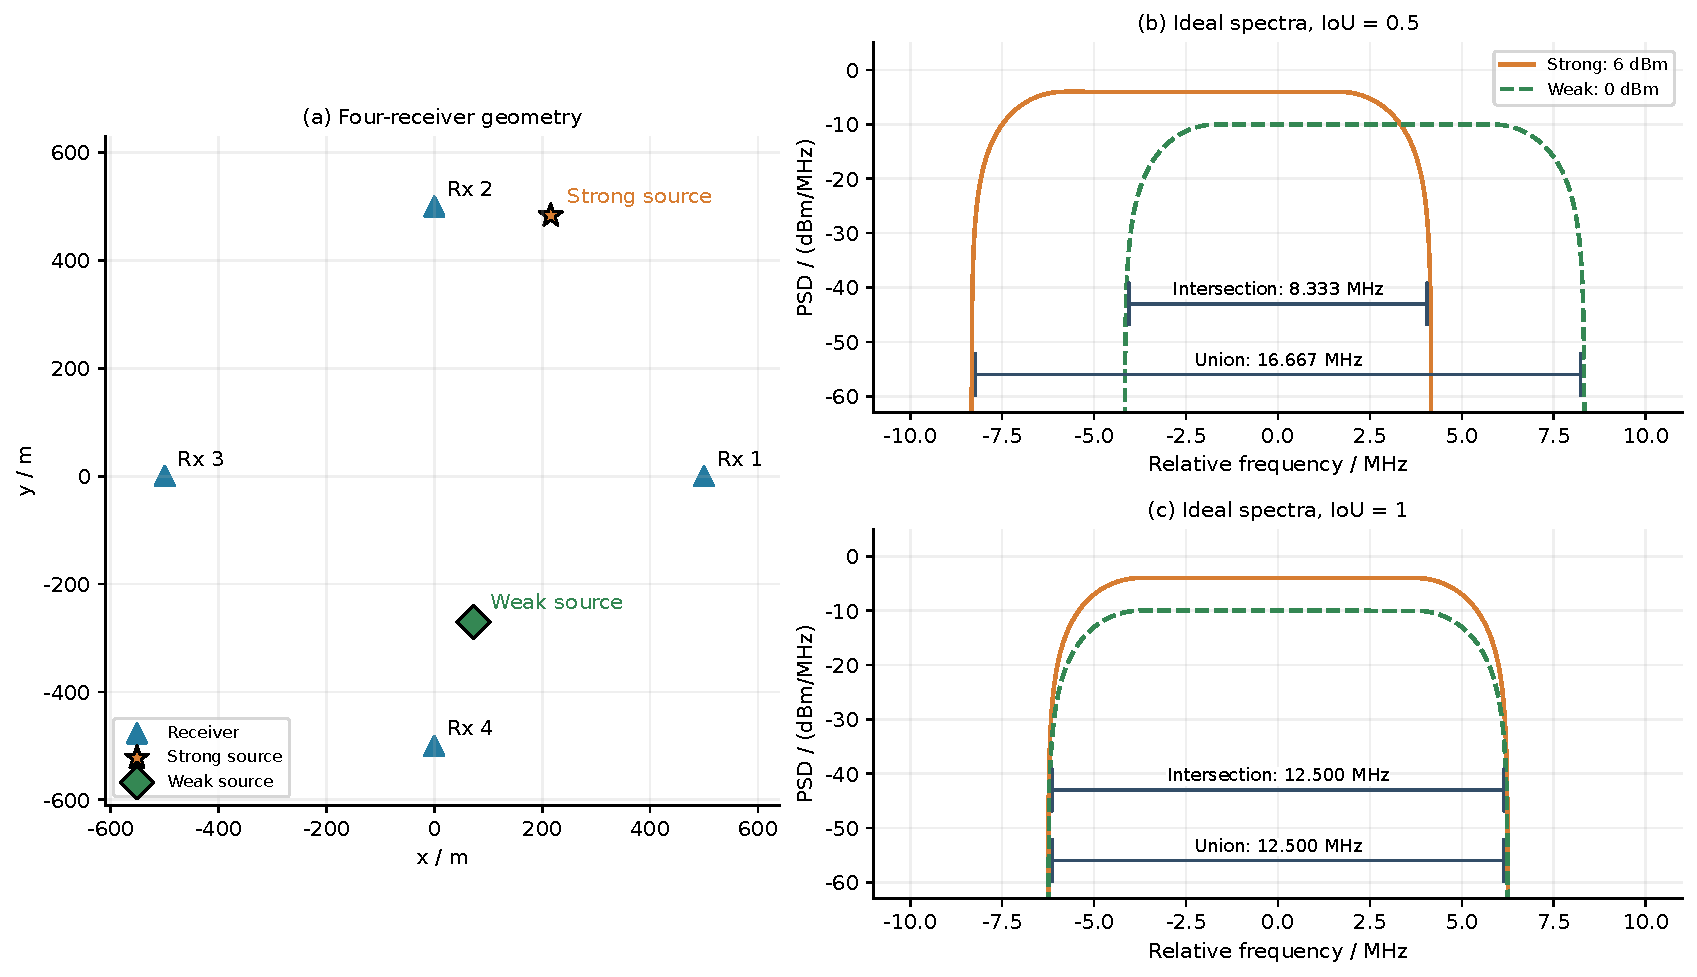
\includegraphics[width=\linewidth]{figures/fig_2_1.pdf}
\caption{Four single-antenna receivers and two spectral-overlap conditions.}\label{fig:2.1}
\begin{minipage}{\linewidth}\small
(a) Four receivers lie on a circle of radius 500 m. The strong and weak sources are at $(215.85,483.29)$ m and $(72.77,-270.30)$ m, respectively, from one simulated scene. (b), (c) Ideal power spectra of root-raised-cosine (RRC) signals with a 10 MHz symbol rate, roll-off 0.25, and 12.5 MHz support width per source. The illustrative powers of 6 dBm and 0 dBm show a 6 dB difference; the ordinate is power spectral density in dBm/MHz. Intersection-over-union (IoU) is the intersection width divided by the union width of the frequency supports, not the area between spectral curves. A center-frequency separation of $12.5/3$ MHz gives intersection and union widths of $25/3$ and $50/3$ MHz, hence IoU = 0.5; coincident centers give IoU = 1. Position ranges and power definitions are given in Table~\ref{tab:3.1}.
\end{minipage}
\end{figure}

% Source block 28
\begin{table}[H]
\centering
\caption{Principal symbols and dimensions.}\label{tab:2.1}
\small
\setlength{\tabcolsep}{4pt}
\renewcommand{\arraystretch}{1.2}
\begin{tabularx}{\linewidth}{Y{0.85}Y{1.35}Y{0.8}}
\toprule
\textbf{Symbol} & \textbf{Meaning} & \textbf{Dimension or unit} \\
\midrule
$\mathbf{r}_\ell,\mathbf{p}_k$ & Receiver and source positions & $2\times1$, m \\
$d_{\ell k},\tau_{\ell k}$ & Propagation distance and delay & m, s \\
$F_s,T_s,T$ & Sampling rate, sampling interval, and observation duration & Hz, s, s \\
$\mathbf{x}_m,\mathbf{s}_m$ & Receiver observations and source coefficients at frequency $m$ & $L\times1$, $K\times1$ \\
$\mathbf{A}_m$ & Response matrix parameterized by position & $L\times K$ \\
$\Pi_m^\perp$ & Orthogonal projector onto the complement of the response column space & $L\times L$ \\
$\mathbf{D}_m$ & Derivative of the mean with respect to real position parameters & $L\times2K$ \\
$\mathbf{J}_{\theta}^{\mathrm{eff}}$ & Position information after eliminating unknown waveforms & $2K\times2K$, m$^{-2}$ \\
\bottomrule
\end{tabularx}
\end{table}

% Source block 30
Superscripts $T$, $H$, and $\dagger$ denote transpose, conjugate transpose, and the Moore--Penrose pseudoinverse, respectively; $\|\cdot\|$ denotes the Euclidean norm.

% Source block 31
\subsection{Received-signal model}\label{sec:2.2}

% Source block 32
Following the wideband joint-localization model in\cite{ref05}, let $s_k(t)$ be the continuous complex baseband signal of source $k$. The propagation distance, delay, and amplitude attenuation are
% Source block 33
\begin{equation}\label{eq:2.2}
d_{\ell k}=\|\mathbf{p}_k-\mathbf{r}_\ell\|, \qquad \tau_{\ell k}=\frac{d_{\ell k}}{c}, \qquad g_{\ell k}=\frac{1}{d_{\ell k}}.
\end{equation}

% Source block 34
A common attenuation constant is absorbed into $s_k(t)$. With $N$ samples per receiver, the observation model is
% Source block 35
\begin{equation}\label{eq:2.3}
x_\ell[n] =\sum_{k=1}^{K}g_{\ell k} s_k(nT_s-\tau_{\ell k})+w_\ell[n], \quad n=0,\ldots,N-1, \qquad w_\ell[n]\sim\mathcal{CN}(0,\sigma_t^2).
\end{equation}

% Source block 36
Here, $T_s=1/F_s$, $T=NT_s$ is the observation duration, and $c$ is the propagation speed. The complex noise satisfies $\mathbb{E}|w_\ell[n]|^2=\sigma_t^2$, with variance $\sigma_t^2/2$ in each real and imaginary component. The two simulated sources use independent binary phase-shift keying (BPSK) data, symbol timing, and initial phase, followed by RRC pulse shaping. The localization algorithms do not use the transmitted bits or true individual source spectra. Statistical independence of the sources does not make their finite-record cross terms identically zero.

% Source block 37
The discrete Fourier transform (DFT) is normalized by $N$:
% Source block 38
\begin{equation}\label{eq:2.4}
X_{\ell m} =\frac{1}{N}\sum_{n=0}^{N-1}x_\ell[n]e^{-j2\pi mn/N}, \qquad \sigma_f^2=\frac{\sigma_t^2}{N}.
\end{equation}

% Source block 39
\begin{samepage}
Both positive and negative frequencies are retained, with $f_m$ denoting signed baseband frequency. Under a frequency-domain approximation that neglects observation-window edge effects\cite{ref04,ref05}, stacking the receiver observations at each frequency gives
% Source block 40
\begin{equation}\label{eq:2.5}
\mathbf{x}_m =\mathbf{A}_m(\theta)\mathbf{s}_m +\mathbf{n}_m, \qquad \mathbf{n}_m\sim\mathcal{CN}(\mathbf{0},\sigma_f^2\mathbf{I}_L),
\end{equation}
% Source block 41
\begin{equation}\label{eq:2.6}
[\mathbf{a}_m(\mathbf{p}_k)]_\ell =\frac{e^{-j2\pi f_m d_{\ell k}/c}}{d_{\ell k}}, \qquad \mathbf{A}_m=[\mathbf{a}_m(\mathbf{p}_1),\ldots,\mathbf{a}_m(\mathbf{p}_K)].
\end{equation}
\end{samepage}

% Source block 42
The carrier-phase convention is $f_c=0$. The likelihood and information analysis below refer to the frequency-domain model in (\ref{eq:2.5}).

% Source block 43
The source coefficients $\mathbf{s}_m$ are fitted separately at each frequency, while positions are shared across frequencies. Gains are not estimated in this appendix. Arbitrary gains varying independently at every receiver and frequency could absorb delay phases; the frequency-shared gains in the main text do not constitute that degenerate case.

% Source block 44
\subsection{Waveform elimination and the multisource DPD objective}\label{sec:2.3}

% Source block 45
Under this frequency-domain model and equal-variance white noise, the negative log-likelihood is proportional to the total squared fitting residual after parameter-independent terms are removed. The concentrated least-squares position estimate is
% Source block 46
\begin{equation}\label{eq:2.7}
\widehat{\theta} = \arg\min_{\theta\in\Omega^K} \min_{\{\mathbf{s}_m\}} \sum_m \|\mathbf{x}_m-\mathbf{A}_m(\theta)\mathbf{s}_m\|^2, \quad \Omega=[-1000,1000]^2\ \mathrm{m}^2.
\end{equation}

% Source block 47
For fixed positions, the minimum-norm least-squares (LS) estimate of the source coefficients is
% Source block 48
\begin{equation}\label{eq:2.8}
\widehat{\mathbf{s}}_m=\mathbf{A}_m^\dagger\mathbf{x}_m.
\end{equation}

% Source block 49
Define the projectors onto the response column space and its orthogonal complement as
% Source block 50
\begin{equation}\label{eq:2.9}
\Pi_m=\mathbf{A}_m\mathbf{A}_m^\dagger, \qquad \Pi_m^\perp=\mathbf{I}_L-\Pi_m.
\end{equation}

% Source block 51
Substituting the coefficient estimate gives a concentrated objective containing only position parameters\cite{ref05}:
% Source block 52
\begin{equation}\label{eq:2.10}
J(\theta) =\sum_m\|\Pi_m^\perp\mathbf{x}_m\|^2.
\end{equation}

% Source block 53
Exchanging source labels leaves this objective unchanged, so the estimated positions are evaluated as an unordered set. The objective uses propagation relations across all receivers and all frequencies included in the fit, without requiring a separate TDOA estimate for each source. A finite search need not attain its global minimum.

% Source block 54
\subsection{Sequential search and joint updates}\label{sec:2.4}

% Source block 55
Enumerating combinations of $K$ two-dimensional positions becomes costly as the source count increases. The solver initializes sources sequentially, alternates position updates, and periodically searches again for previously estimated sources. When one position is updated, the other positions are fixed. Writing their responses as $\mathbf{B}_m$, define
% Source block 56
\begin{equation}\label{eq:2.11}
\begin{aligned}
&\Pi_{B,m}^\perp =\mathbf{I}-\mathbf{B}_m\mathbf{B}_m^\dagger, \\
& \mathbf{r}_m=\Pi_{B,m}^\perp\mathbf{x}_m, \quad \mathbf{u}_m(\mathbf{p})=\Pi_{B,m}^\perp\mathbf{a}_m(\mathbf{p}).
\end{aligned}
\end{equation}

% Source block 57
Both the new source coefficient and the coefficients of the existing sources are refitted. Eliminating these linear LS variables gives the residual reduction associated with a candidate position:
% Source block 58
\begin{equation}\label{eq:2.12}
Q(\mathbf{p}\mid\mathbf{B}) = \sum_m \frac{|\mathbf{a}_m(\mathbf{p})^H\Pi_{B,m}^\perp\mathbf{x}_m|^2} {\mathbf{a}_m(\mathbf{p})^H\Pi_{B,m}^\perp\mathbf{a}_m(\mathbf{p})}.
\end{equation}

% Source block 59
The denominator is the energy of the projected candidate response, so the score equals the improvement in the joint LS fit. Projection and candidate-response normalization also appear in round-robin localization\cite{ref07}. When $\mathbf{u}_m=\mathbf{0}$, the candidate adds no new direction to the column space and its increment at that frequency is defined as zero. Otherwise,
% Source block 60
\begin{equation}\label{eq:2.13}
0\leq \frac{|\mathbf{u}_m^H\mathbf{r}_m|^2}{\|\mathbf{u}_m\|^2} \leq\|\mathbf{r}_m\|^2.
\end{equation}

% Source block 61
The implementation checks numerical scales at degenerate frequencies and normalizes scores by the total observation energy $E_x=\sum_m\|\mathbf{x}_m\|^2$. This normalization preserves candidate ordering within a record.

The complete localization methods are defined in Table~\ref{tab:methods}. Conventional DPD selects spatial-spectrum peaks directly. Methods A, B, C, and D use the concentrated LS objective and differ mainly in candidate search. AP denotes alternating projection.

\begin{table}[H]
\centering
\caption{Localization methods and candidate-search strategies.}\label{tab:methods}
\small
\setlength{\tabcolsep}{4pt}
\renewcommand{\arraystretch}{1.2}
\begin{tabularx}{\linewidth}{Y{0.85}Y{1.05}Y{1.1}}
\toprule
\textbf{Method} & \textbf{Candidate search} & \textbf{Objective and position updates} \\
\midrule
Conventional DPD & Largest eigenvalue of the delay-compensated correlation matrix; coarse-to-fine search & Two peaks selected and refined separately, without sequential projection \\
A: Multistart AP & Coarse grid and multiple initializations & Concentrated LS, L-BFGS-B, alternating updates, and cyclic search \\
B: Standard regional search & Subdivision by current score, with global exploration & Same as A \\
C: Response-guided search & B with additional ranking by response variation & Same as A \\
D: Supplementary global search & Complete B, then a 5 m scan and refinement of the top 5 candidates for each source & Same concentrated LS objective, followed by 2 local alternating-update rounds \\
\bottomrule
\end{tabularx}
\end{table}

Conventional DPD scores positions using the largest eigenvalue of a delay-compensated correlation matrix normalized by receiver energies. Coarse-to-fine peak selection and separate refinement produce the position estimates. Its comparison with A, B, and C therefore concerns complete solution procedures.

Methods A, B, and C use the same initial candidate search based on conventional DPD, whose cost is included in total processing time. They use 5 initializations, at most 5 alternating-update rounds, and at most 30 iterations per local optimization. Previously estimated sources are searched again in rounds 3 and 5. B and C subdivide at most 48 cells at a time and reserve one in every 4 search steps for global exploration. C uses the response-variation measure defined in Section~\ref{sec:2.5.3}, with ranking weight fixed at 0.25.

The mixed observations are first normalized by receiver RMS to generate largest-eigenvalue spectral candidates. A--C then use the concentrated LS objective on raw observations for multiple starts, source-wise searches, continuous refinement, and joint waveform refitting. Searches are not restricted to neighborhoods of the initial positions, and rounds 3 and 5 include renewed searches. D adds a further full-region scan. Initialization may affect finite-budget estimates, but its effect has not been isolated in the existing comparisons.

% Source block 62
\begin{figure}[!htbp]
\centering
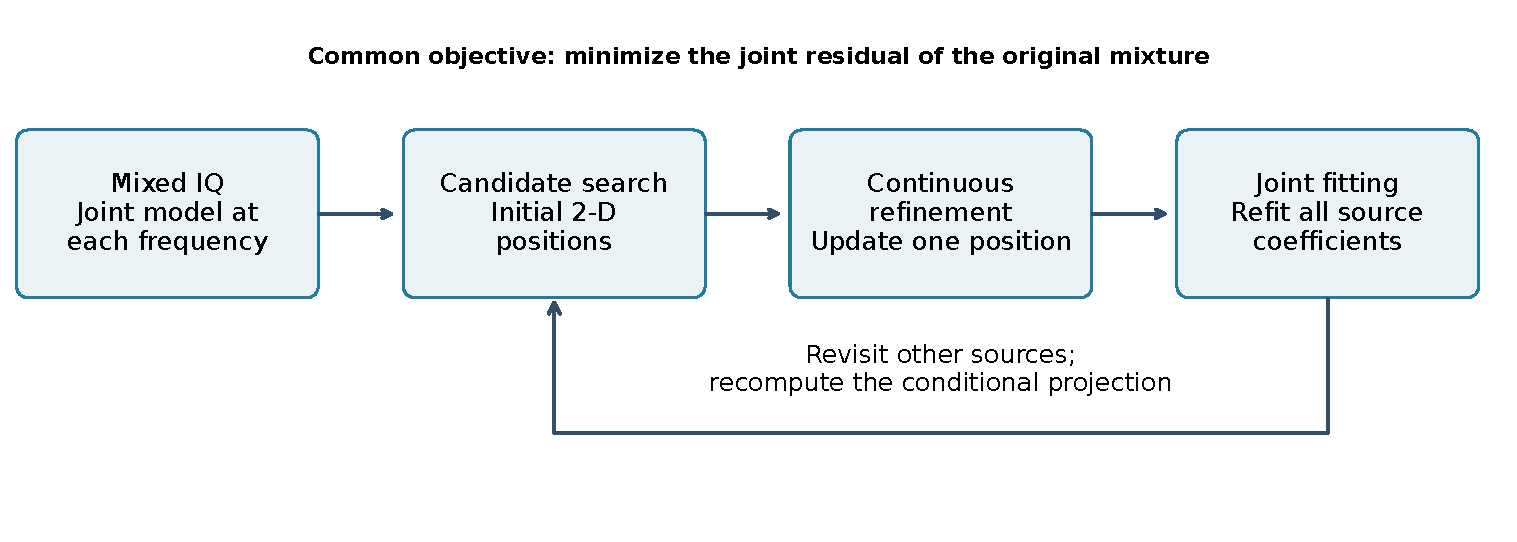
\includegraphics[width=\linewidth]{figures/fig_2_2.pdf}
\caption{Common solution procedure for the joint objective.}\label{fig:2.2}
\begin{minipage}{\linewidth}\small
Candidate search supplies initial positions, continuous optimization refines positions, and all frequency-domain source coefficients are refitted. The conditional projector is recomputed on each revisit. A, B, C, and D share the concentrated LS objective but differ in candidate coverage and cost.
\end{minipage}
\end{figure}

% Source block 65
After an accepted position update, all source coefficients are refitted before another position is updated. Retaining the solution with the smaller joint residual makes accepted residuals nonincreasing, but does not ensure convergence to a basin near the true positions.

To assess insufficient candidate coverage, method D adds one global-update sweep to the output of the complete method B. For each source in turn, it fixes the other position, evaluates (\ref{eq:2.12}) on a 5 m grid over the entire search region, and continuously refines the top 5 candidates. After both positions have been updated, it performs two local alternating-update rounds. Each step retains the solution with the smaller joint residual. Only observations and current estimates are used; true positions are reserved for evaluation.

% Source block 66
\subsection{Theoretical and algorithmic difficulties}\label{sec:2.5}

% Source block 67
\subsubsection{Local identifiability and global search}\label{sec:2.5.1}

% Source block 68
If $K\geq L$ and the response matrix has full row rank, freely fitted coefficients at each frequency can reproduce any observation, making the concentrated objective degenerate. With $L=4$ and $K=2$, a full-column-rank response leaves two complex residual dimensions per frequency. Local position identifiability still depends on the response derivatives.

% Source block 69
Let $\mathbf{D}_m=\partial(\mathbf{A}_m\mathbf{s}_m)/\partial\theta^T$, with source coefficients held fixed during differentiation. If the response has full column rank locally and the noise covariance is known and parameter independent, eliminating the unknown complex waveforms gives the equivalent position information\cite{ref05,ref10}
% Source block 70
\begin{equation}\label{eq:2.14}
\boxed{ \mathbf{J}_\theta^{\mathrm{eff}} = \frac{2}{\sigma_f^2} \operatorname{Re} \sum_m \mathbf{D}_m^H\Pi_m^\perp\mathbf{D}_m }.
\end{equation}

% Source block 71
When this matrix is positive definite, its inverse gives the Cram\'er--Rao lower bound (CRLB) for regular, locally unbiased position estimation. The bound describes accuracy near the true positions, not whether a solver reaches that neighborhood. Distant local optima and threshold effects require separate analysis\cite{ref11}.

% Source block 72
\subsubsection{Projection loss and strong-source position error}\label{sec:2.5.2}

% Source block 73
At one frequency, let $\mathbf{a}_s$ and $\mathbf{a}_w$ be the strong- and weak-source responses. With the true strong-source response fixed, define $\Pi_s^\perp=\mathbf{I}-\mathbf{a}_s\mathbf{a}_s^H/\|\mathbf{a}_s\|^2$. The response correlation and retained weak-source energy fraction are
% Source block 74
\begin{equation}\label{eq:2.15}
\rho =\frac{\mathbf{a}_s^H\mathbf{a}_w}{\|\mathbf{a}_s\|\|\mathbf{a}_w\|}, \qquad \eta =\frac{\|\Pi_s^\perp\mathbf{a}_w\|^2}{\|\mathbf{a}_w\|^2} =1-|\rho|^2.
\end{equation}

% Source block 75
When the responses are similar, removing the strong source also removes some weak-source energy. Broadband retention must be weighted by the actual weak-source energy at each frequency; one frequency cannot represent the entire observation. For a fixed projector, the noise covariance is $\sigma_f^2\Pi_s^\perp$. In an orthonormal basis of the retained subspace, equal-variance LS remains applicable.

% Source block 76
Let $\delta\mathbf{p}_s$ be the strong-source position error, $\mathbf{H}_{s,m}=\partial\mathbf{a}_m(\mathbf{p}_s)/\partial\mathbf{p}_s^T$, and $s_{sm}$ the source coefficient at frequency $m$. For small position errors, the leading term of residual strong-source energy is
% Source block 77
\begin{equation}\label{eq:2.16}
E_{\mathrm{leak}} \approx \sum_m |s_{sm}|^2 \|\Pi_{s,m}^\perp\mathbf{H}_{s,m}\delta\mathbf{p}_s\|^2.
\end{equation}

% Source block 78
Leakage depends on strong-source power and the direction of the position error. A strong-source estimate can therefore satisfy the localization success criterion while still distorting the weak-source score. Because the projection position is usually estimated from the same observations, its error and the residual are statistically dependent.

% Source block 79
\subsubsection{Sampling narrow peaks and retaining candidates}\label{sec:2.5.3}

% Source block 80
Equation~(\ref{eq:2.13}) bounds the incremental score, but the normalized projected-response direction can still change rapidly with position when its norm is small. Hold the other positions fixed and let $\delta$ be a two-dimensional displacement. Near a smooth local maximum $\mathbf{p}_\star$, with $\mathbf{H}_\star=-\nabla^2Q(\mathbf{p}_\star)\succ0$,
% Source block 81
\begin{equation}\label{eq:2.17}
Q(\mathbf{p}_\star+\delta) =Q(\mathbf{p}_\star) -\frac12\delta^T\mathbf{H}_\star\delta +O(\|\delta\|^3).
\end{equation}

% Source block 82
For a square grid with spacing $h$, the nearest grid point satisfies $\|\delta\|^2\leq h^2/2$. Where the local expansion is valid,
% Source block 83
\begin{equation}\label{eq:2.18}
Q(\mathbf{p}_\star)-Q(\mathbf{p}_{\mathrm{grid}}) \leq\frac{\lambda_{\max}(\mathbf{H}_\star)h^2}{4}+O(h^3).
\end{equation}

% Source block 84
Even when a high peak exists near the true position, sampling loss can rank its nearest grid point below distant candidates. Uniformly reducing grid spacing limits this loss, but the number of evaluations in two dimensions grows as $h^{-2}$. The search must determine which regions merit further evaluations within the available budget.

% Source block 85
One regional selection rule considered here uses spatial variation of the projected response. Let $M$ be the number of frequencies used for scoring, and let $\partial_i$ denote differentiation with respect to coordinate $p_i$. With the other positions fixed, define
% Source block 86
\begin{equation}\label{eq:2.19}
\zeta(\mathbf{p}) =\frac{1}{M}\sum_{m=1}^{M}\sum_{i\in\{x,y\}} \left[ \frac{\|\partial_i\mathbf{u}_m\|^2}{\|\mathbf{u}_m\|^2} - \frac{|\mathbf{u}_m^H\partial_i\mathbf{u}_m|^2}{\|\mathbf{u}_m\|^4} \right].
\end{equation}

% Source block 87
This measure quantifies local sensitivity of the response direction after removing changes in overall amplitude and phase. Method C multiplies it by the squared cell half-width, converts it to a rank, and combines this rank with the score rank. It does not directly use the observed residual, so rapid response variation need not indicate a high-scoring candidate. Its benefit is assessed under matched time budgets.

\subsubsection{Regional score upper bound and pruning}\label{sec:region-bound}

To determine whether an incompletely sampled region may contain a higher score, consider a conditional upper bound with all other sources fixed. A square cell $\mathcal C$ has center $\mathbf p_c$ and half-width $h$, so every point in it lies within $\Delta_{\mathcal C}=\sqrt{2}h$ of the center. The numerical search floors receiver distances at $d_0=1$ m to avoid the $1/d$ singularity; the bound uses the same response. Write $d_\ell^c=\max(\|\mathbf p_c-\mathbf r_\ell\|,d_0)$ and $d_{\ell,-}=\max(d_\ell^c-\Delta_{\mathcal C},d_0)$. Bounds on distance changes and complex-exponential phase differences give the following bound on the response change at one receiver:
\begin{equation}\label{eq:response-bound}
\begin{aligned}
\varepsilon_{\ell m}
&=\frac{\Delta_{\mathcal C}}{d_\ell^c d_{\ell,-}}
+\frac{2}{d_\ell^c}\sin\!\left[\frac12\min\!\left(\pi,\frac{2\pi|f_m|\Delta_{\mathcal C}}{c}\right)\right],\\
\varepsilon_m&=\left(\sum_{\ell=1}^{L}\varepsilon_{\ell m}^2\right)^{1/2}.
\end{aligned}
\end{equation}

Orthogonal projection cannot increase a vector norm, so $\|\mathbf u_m(\mathbf p)-\mathbf u_m(\mathbf p_c)\|\leq\varepsilon_m$. Denote the projected center response by $\mathbf u_m^c=\mathbf u_m(\mathbf p_c)$ and define
\begin{equation}\label{eq:cone-parameters}
t_m=\min\!\left(1,\frac{\varepsilon_m}{\|\mathbf u_m^c\|}\right),\qquad
v_m=\frac{|(\mathbf u_m^c)^H\mathbf r_m|}{\|\mathbf u_m^c\|\,\|\mathbf r_m\|}.
\end{equation}

For $t_m<1$, the response direction deviates by at most $\arcsin t_m$. Bounding its angle with the residual gives the following regional upper bound on the normalized score:
\begin{equation}\label{eq:cell-upper}
\begin{aligned}
\frac{Q(\mathbf p\mid\mathbf B)}{E_x}&\leq U(\mathcal C)
=\frac{1}{E_x}\sum_m\|\mathbf r_m\|^2 H(v_m,t_m),\quad \mathbf p\in\mathcal C,\\
H(v,t)&=\begin{cases}
\bigl(v\sqrt{1-t^2}+t\sqrt{1-v^2}\bigr)^2,&t<\sqrt{1-v^2},\\
1,&t\geq\sqrt{1-v^2}.
\end{cases}
\end{aligned}
\end{equation}

A zero residual contributes zero. At a degenerate projected center response, the residual energy at that frequency is used as the upper bound. A cell can be pruned when $U(\mathcal C)$ is below the best score already found; otherwise, cells with larger upper bounds can be subdivided first. Whether this bound is tight enough, and whether its evaluation is cheaper than sampling additional positions, are empirical questions. Section~\ref{sec:3.10} compares it with score-prioritized subdivision and uniform and shifted grids.

% Source block 88
The objective is to detect weak-source candidates missed by coarse search within a fixed observation and computational budget, while reducing the effects of strong-source errors through joint position updates.

% Source block 90
\section{Experiments with known relative gains}\label{sec:3}

All data in this appendix are from the existing experiments with known relative gains. The original comparison, new-layout comparison, and selected diagnostics remain separate, with unchanged denominators, success criteria, and processing times. They do not establish performance for the unknown-gain model.

% Source block 91
\subsection{Simulation setup}\label{sec:3.1}

% Source block 92
Methods A, B, and C are first compared on 32 independent layouts, followed by analysis of their failures. Complete methods B and D are then compared on six new layouts. The regional-bound comparison uses 24 fixed diagnostic records and updates only the weak-source position. These three sets are analyzed separately. Section~\ref{sec:3.7} provides an additional frequency-domain illustration of the projection mechanism.

% Source block 93
\begin{table}[H]
\centering
\caption{Simulation parameters and settings for the first method comparison.}\label{tab:3.1}
\small
\setlength{\tabcolsep}{4pt}
\renewcommand{\arraystretch}{1.2}
\begin{tabularx}{\linewidth}{Y{0.65}Y{1.35}}
\toprule
\textbf{Parameter} & \textbf{Setting} \\
\midrule
Receiver geometry & Four receivers at approximately $(500,0),(0,500),(-500,0),(0,-500)$ m \\
Search region & $[-1000,1000]^2$ m$^2$; continuous source positions \\
Source count and separation & Known $K=2$; source separation at least 300 m; source-to-receiver distance at least 150 m \\
Waveforms & Two independent BPSK/RRC sources; symbol rate 10 MHz; roll-off 0.25 \\
Sampling and record length & $F_s=100$ MHz; $N=4096,16384$ \\
Nominal bandwidth and overlap & 12.5 MHz; spectral-support IoU of 0.5 or 1 \\
Weak-source power & Network-averaged in-band signal-to-noise ratio (SNR) of 3 dB \\
Power difference & Network-averaged received-power difference of 6 or 12 dB \\
Independent layouts and realizations & 32 layouts, with 2 waveform/noise realizations per layout \\
Mixed-source conditions & $32\times2\times2\times2\times2=512$ records \\
Isolated-source controls & 128 isolated weak-source and 128 isolated strong-source records per length \\
Main budget $T_0$ & 3.7216 s for 4096 samples; 11.5376 s for 16384 samples \\
Budget comparison & $0.5T_0,T_0,2T_0$, using the output completed by each deadline \\
\bottomrule
\end{tabularx}
\end{table}

% Source block 95
Short and long records are prefixes of the same continuous waveform and noise streams. Across the two power differences, the weak signal and noise are identical sample by sample; only the strong-source amplitude changes. Layouts are the independent sampling units, and confidence intervals use paired resampling of layout clusters.

% Source block 96
Method parameters are fixed before each comparison. Failure diagnostics from the first set are used to select the supplementary search configuration. The 5 m grid, candidate count, and update rounds for D are fixed before evaluating the six new layouts. Isolated/mixed comparisons preserve the weak signal and noise to measure the additional loss caused by the strong source.

The comparison involving D uses complete executions of B as the baseline, rather than the deadline outputs from the first set. B and D use the same batched double-precision score implementation. The total time for D includes B and the supplementary search. Computation uses an NVIDIA RTX 4070 Ti SUPER, PyTorch 2.8.0, and 4 CPU threads.

% Source block 100
\subsection{Evaluation metrics}\label{sec:3.2}

% Source block 101
Let $\mathcal{P}$ and $\widehat{\mathcal{P}}$ denote the true and estimated position sets. For a success radius $r$, matching first maximizes the number of source pairs within that radius, then breaks ties by squared distance and a fixed deterministic rule. Let $I_{w,j}(r)$ and $I_{s,j}(r)$ indicate successful matches for the weak and strong sources in record $j$. The weak-source and simultaneous two-source success rates are
% Source block 102
\begin{equation}\label{eq:3.1}
\begin{aligned}
&R_w(r)=\frac{1}{n_{\mathrm{rec}}}\sum_{j=1}^{n_{\mathrm{rec}}}I_{w,j}(r), \\
& R_{\mathrm{both}}(r) =\frac{1}{n_{\mathrm{rec}}}\sum_{j=1}^{n_{\mathrm{rec}}}I_{s,j}(r)I_{w,j}(r).
\end{aligned}
\end{equation}

% Source block 103
Here, $n_{\mathrm{rec}}$ is the number of records. The success radius is 2\% of the largest receiver baseline, namely $r=0.02\max_{\ell,q}\|\mathbf{r}_\ell-\mathbf{r}_q\|=20$ m. Root-mean-square error (RMSE), the 95th percentile (P95), and the error cumulative distribution function (CDF) use a separate minimum-squared-distance assignment and retain all matched errors. The two assignments serve success counting and distance-error statistics, respectively.

% Source block 104
Set error is measured by the generalized optimal sub-pattern assignment (GOSPA) distance\cite{ref12}, with $p=2,\alpha=2,\kappa=100$ m. Its partial-assignment form is
% Source block 105
\begin{equation}\label{eq:3.2}
d_{\mathrm G}^2(\mathcal{P},\widehat{\mathcal{P}}) = \min_{\gamma} \left[ \sum_{(i,j)\in\gamma}\|\mathbf{p}_i-\widehat{\mathbf{p}}_j\|^2 +\frac{\kappa^2}{2}(K+\widehat K-2|\gamma|) \right],
\end{equation}

% Source block 106
Here, $\gamma$ is a one-to-one partial assignment. The GOSPA cutoff $\kappa$ is distinct from the 20 m success radius. Reported GOSPA values are means of the per-record distance $d_{\mathrm G}$; RMSE is the square root of the mean untruncated squared distance error.

% Source block 107
Total online processing time includes the shared candidate front end, propagation-model scoring, projection, search, and continuous refinement. The three budget snapshots come from the same run trajectory and retain the original layout grouping in the analysis.

% Source block 108
\subsection{The weak source in isolation and in a mixture}\label{sec:3.3}

% Source block 109
\begin{figure}[!htbp]
\centering
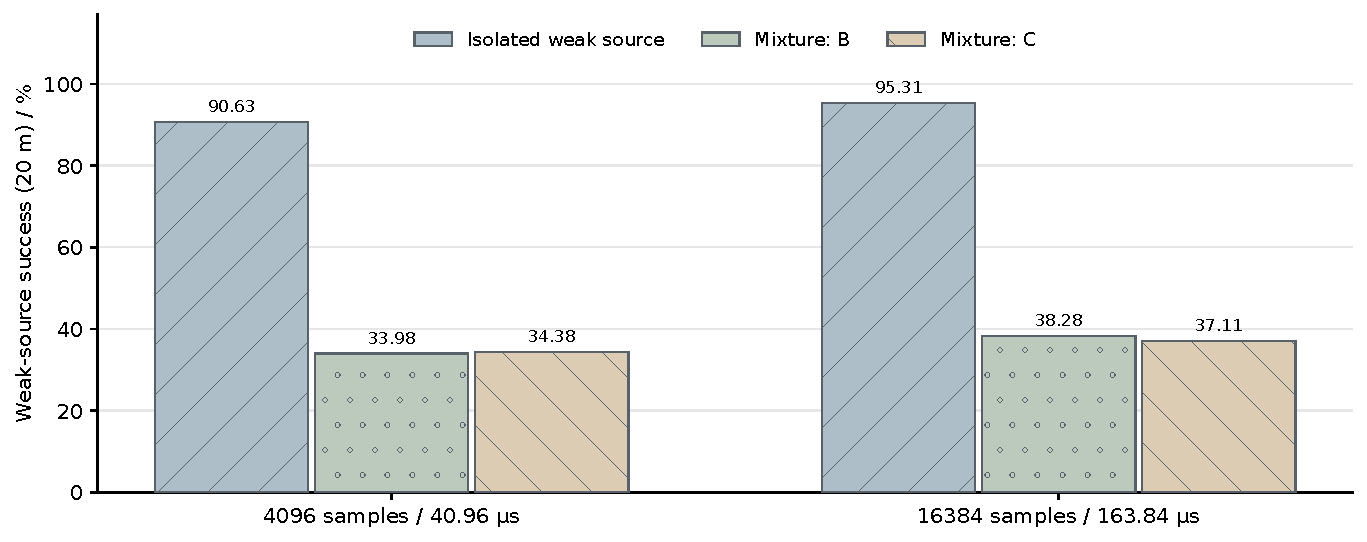
\includegraphics[width=\linewidth]{figures/fig_3_1.pdf}
\caption{Isolated and mixed observations with the same weak signal and noise.}\label{fig:3.1}
\begin{minipage}{\linewidth}\small
Each length has 128 isolated weak-source records and 256 mixed conditions. The two power differences in the mixtures share the corresponding weak signal. Mixed-source results use the main budget $T_0$ and a 20 m success radius.
\end{minipage}
\end{figure}

% Source block 112
\begin{table}[H]
\centering
\caption{Weak-source success counts in isolated and mixed observations.}\label{tab:3.3}
\small
\setlength{\tabcolsep}{4pt}
\renewcommand{\arraystretch}{1.2}
\begin{tabularx}{\linewidth}{Y{0.6}Y{1.4}Y{1}Y{1}}
\toprule
\textbf{Samples} & \textbf{Isolated weak source (shared reference)} & \textbf{Mixed, B} & \textbf{Mixed, C} \\
\midrule
4096 & 116/128 (90.625\%) & 87/256 (33.984\%) & 88/256 (34.375\%) \\
16384 & 122/128 (95.313\%) & 98/256 (38.281\%) & 95/256 (37.109\%) \\
\bottomrule
\end{tabularx}
\end{table}

% Source block 114
Isolated weak-source success rates are 90.63\% and 95.31\% for the two lengths. Adding the strong source reduces the rates of B and C to approximately 34\% to 38\%. Because the weak signal and noise are unchanged, this difference measures the additional loss from the strong source. Increasing the record length from 4096 to 16384 samples improves weak-source success in the mixture, but a substantial gap from isolated-source performance remains.

% Source block 115
Relative source strengths at individual receivers depend on geometry and transmit power. The network-average definition does not require one source to dominate at every receiver. Source competition must therefore be examined through the actual responses; a single global power ratio cannot predict success or failure.

% Source block 116
\subsection{Sequential processing and candidate ranking}\label{sec:3.4}

% Source block 117
\begin{figure}[!htbp]
\centering
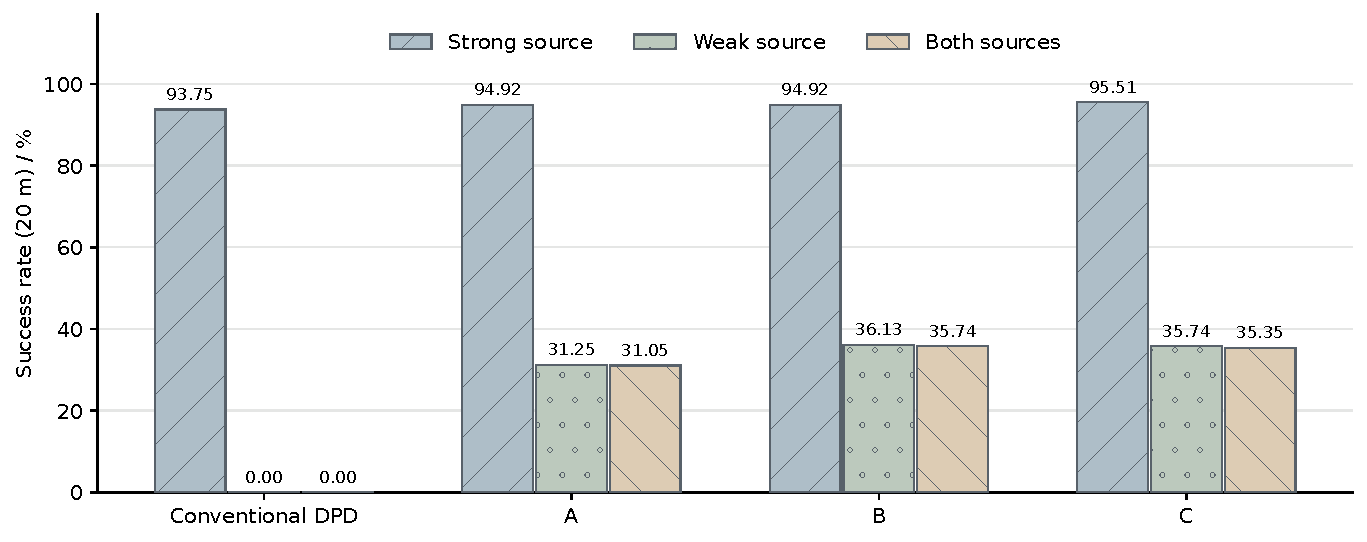
\includegraphics[width=\linewidth]{figures/fig_3_2.pdf}
\caption{Complete-method comparison at the main budget.}\label{fig:3.2}
\begin{minipage}{\linewidth}\small
Results combine both record lengths, giving 512 mixed conditions per method, with a 20 m success radius. A, B, and C share sequential projection and joint updates. Method D is evaluated separately on new layouts in Section~\ref{sec:3.9}.
\end{minipage}
\end{figure}

% Source block 120
\begin{table}[H]
\centering
\caption{Aggregate results at the main budget $T_0$.}\label{tab:3.4}
\small
\setlength{\tabcolsep}{4pt}
\renewcommand{\arraystretch}{1.2}
\begin{tabularx}{\linewidth}{Y{1.15}Y{1.0}Y{1.1}Y{1.0}Y{1.05}Y{0.85}Y{0.85}}
\toprule
\textbf{Method} & \textbf{Weak success} & \textbf{Both sources successful} & \textbf{Strong success} & \textbf{Mean GOSPA / m} & \textbf{RMSE / m} & \textbf{P95 / m} \\
\midrule
Conventional DPD & 0.00\% & 0.00\% & 93.75\% & 101.73 & 807.21 & 1684.03 \\
A & 31.25\% & 31.05\% & 94.92\% & 64.16 & 259.85 & 616.25 \\
B & 36.13\% & 35.74\% & 94.92\% & 60.46 & 256.71 & 612.58 \\
C & 35.74\% & 35.35\% & 95.51\% & 61.36 & 242.01 & 579.53 \\
\bottomrule
\end{tabularx}
\end{table}

% Source block 122
Conventional DPD usually localizes the strong source, but none of its weak-source estimates meets the 20 m criterion. With sequential projection and joint updates, A, B, and C achieve weak-source success rates from 31.25\% to 36.13\%. C exceeds A by 4.49 percentage points, with a 95\% paired interval of $[0.59,8.79]$ percentage points from resampling the 32 layouts. Relative to B, C is lower by 0.39 percentage points, with an interval of $[-5.27,3.91]$ percentage points.

% Source block 123
In paired comparisons, C recovers 22 weak-source failures of B but fails on 24 records where B succeeds, giving a net loss of 2 successes. C has lower RMSE, while GOSPA and the 20 m success rate do not improve. Ranking by response variation therefore shows no consistent benefit over the standard regional search B.

% Source block 124

% Source block 125
\subsection{Conditional scores and failure analysis}\label{sec:3.5}

% Source block 126
Conditional scores are examined for the 512 mixed records of B, with its main-budget outputs held fixed. For the 327 weak-source failures, the comparisons are: the true weak position versus the returned position under the estimated strong position; the same two positions under the true strong position; and the true position pair versus the returned pair under the joint objective. True positions are used only for diagnosis, not for candidate generation.

% Source block 127
\begin{table}[H]
\centering
\caption{Conditional-score analysis of all failed records.}\label{tab:3.5}
\small
\setlength{\tabcolsep}{4pt}
\renewcommand{\arraystretch}{1.2}
\begin{tabularx}{\linewidth}{Y{0.65}Y{0.8}Y{1.15}Y{1.2}Y{1.2}}
\toprule
\textbf{Samples} & \textbf{Weak failures of B} & \textbf{True weak score higher: estimated strong} & \textbf{True weak score higher: true strong} & \textbf{True pair gives better joint fit} \\
\midrule
4096 & 169 & 147 & 159 & 158 \\
16384 & 158 & 145 & 155 & 155 \\
Total & 327 & 292 & 314 & 313 \\
\bottomrule
\end{tabularx}
\end{table}

% Source block 129
In 292 of 327 failures (89.30\%), the true weak-source position already has a higher score than the returned position, without changing the estimated strong position or score function. Local refinement initialized at the true weak position finds a higher-scoring solution within 20 m in 295 records. These counts can overlap. Most failed records therefore contain a better position that the solver did not find.

% Source block 130
Of the 35 records without a score advantage at the true weak position under the estimated strong position, 22 gain that advantage when the true strong position is substituted. In one of these records, the original strong-source error is already below 20 m. The success radius is thus not a suitable stopping threshold for strong-source refinement: smaller errors can still affect the weak-source score.

% Source block 131
The true position pair gives a smaller joint residual in 313 of the 327 failures. For the remaining records, scores at the true positions alone do not establish a search failure; local estimation bias and convergence to an incorrect basin must be distinguished. Denser-search comparisons further assess the effect of candidate coverage.

% Source block 132
\begin{figure}[!htbp]
\centering
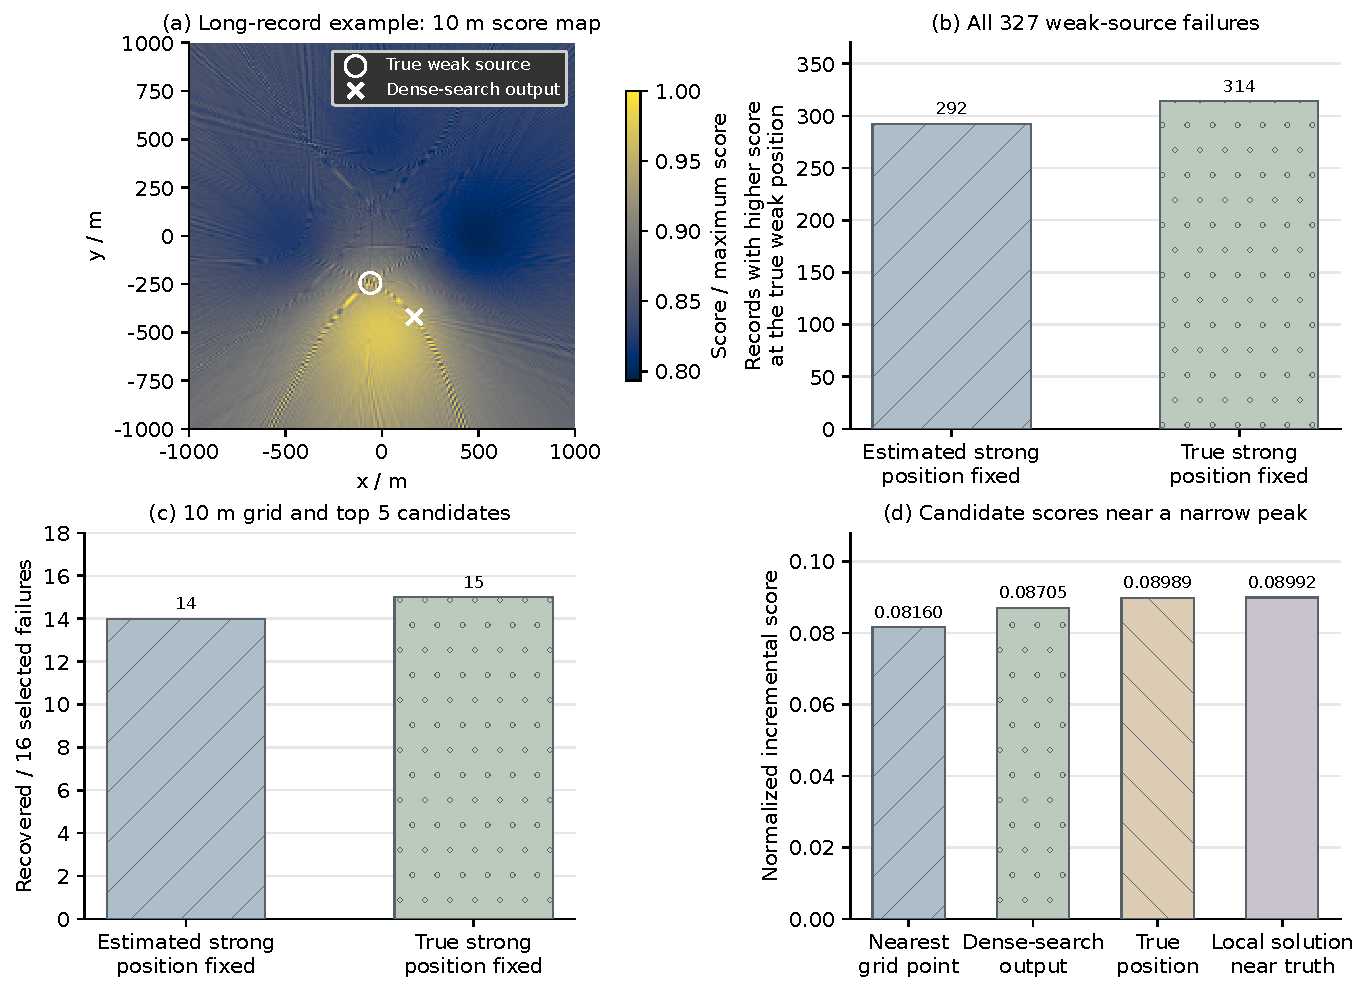
\includegraphics[width=.92\linewidth]{figures/fig_3_3.pdf}
\caption{Score structure and diagnosis of missed candidates.}\label{fig:3.3}
\begin{minipage}{\linewidth}\small
(a) Auxiliary long-record example, IoU = 0.5 and $N=65536$: a 10 m score map over the full region, with the true weak position and dense-search output. This example is excluded from statistics for the two main record lengths. (b) Conditional scores for all 327 weak-source failures of B. (c) Recovery within 20 m among 16 previously selected failures; all 8 historical controls also meet 20 m after the update. (d) A narrow-peak case with $N=4096$, IoU = 1, and a 12 dB power difference: scores at four types of position, with the true strong position fixed.
\end{minipage}
\end{figure}

% Source block 135
\subsection{Dense search and missed narrow peaks}\label{sec:3.6}

% Source block 136
The search diagnosis retains 24 records previously selected under a 100 m criterion; it does not resample the current 327 failures. The records cover four layouts and eight strata defined by length, overlap, and power difference, with two historical failures and one historical control per stratum. All 16 historical failures initially exceed 20 m. Of the 8 controls, only 6 initially satisfy 20 m; the other errors are 61.42 m and 63.37 m. The two fixed groups are retained, and updated outputs are evaluated at 20 m throughout. The diagnostic search fixes the strong-source position and re-estimates the weak source using a full-region 10 m scan, the top 5 candidates, and continuous refinement.

% Source block 137
\begin{table}[H]
\centering
\caption{Search diagnosis on the fixed records.}\label{tab:3.6}
\small
\setlength{\tabcolsep}{4pt}
\renewcommand{\arraystretch}{1.2}
\begin{tabularx}{\linewidth}{Y{1}Y{0.6}Y{1.15}Y{1.1}Y{1.15}}
\toprule
\textbf{Group} & \textbf{Records} & \textbf{Weak successes: estimated strong fixed} & \textbf{Weak successes: true strong fixed} & \textbf{Both successful: initialized at true pair} \\
\midrule
Historical failures & 16 & 14 & 15 & 16 \\
Historical controls & 8 & 8 & 8 & 8 \\
\bottomrule
\end{tabularx}
\end{table}

% Source block 139
Keeping the estimated strong-source position fixed, denser search recovers 14 of the 16 selected failures. These records can be recovered by changing the search, but this recovery fraction from purposively selected cases does not estimate recovery across all failures.

% Source block 140
The two remaining cases have different causes. In the coupling case with 4096 samples, IoU = 1, and a 6 dB power difference, the original strong-source error is 558.73 m. Holding that estimate fixed leaves a weak-source error of 1095.56 m after dense search. Substituting the true strong position reduces it to 0.828 m, directly demonstrating position coupling in this case.

% Source block 141
In the narrow-peak case with 4096 samples, IoU = 1, and a 12 dB power difference, the strong-source error is only 0.073 m, yet the 10 m search returns a weak-source error of approximately 125.48 m. With the true strong position fixed, the scores are as follows.

% Source block 142
\begin{table}[H]
\centering
\caption{Scores in a case with a missed narrow peak.}\label{tab:3.7}
\small
\setlength{\tabcolsep}{4pt}
\renewcommand{\arraystretch}{1.2}
\begin{tabularx}{\linewidth}{Y{1.1}Y{1}Y{0.9}}
\toprule
\textbf{Position} & \textbf{Normalized incremental score} & \textbf{Distance from true weak source} \\
\midrule
Nearest 10 m grid point & 0.08159913 & 4.523 m \\
Dense-search output & 0.08704823 & 125.36 m \\
True weak position & 0.08989170 & 0 m \\
Local solution near truth & 0.08992482 & 0.803 m \\
\bottomrule
\end{tabularx}
\end{table}

% Source block 144
The nearest grid point is only 4.523 m from the true position but scores below the distant returned point. Local refinement from the correct region reaches submeter error, yet the 10 m grid with five retained candidates omits that region. This behavior is consistent with the sampling loss and ranking changes described by (\ref{eq:2.17}) and (\ref{eq:2.18}).

% Source block 145
Grid spacing and candidate count are also compared on these 24 records. With the estimated strong position fixed and the same batched score implementation, a 10 m grid with 5 candidates recovers 14 of 16 historical failures. Increasing the count to 32 still recovers 14, whereas a 5 m grid with 5 candidates recovers 15. All three configurations bring the 8 historical controls within 20 m, including the 2 that initially exceed that radius. Mean supplementary weak-source search times over the 16 failures are 2.95, 3.61, and 11.29 s, respectively, excluding the preceding strong-source estimation. For these records, retaining more candidates does not replace finer spatial sampling.

In a separate auxiliary diagnosis of 16 selected long-record conditions, changing the search while holding the score fixed increases the number of weak sources recovered within 20 m from 3 to 8. This set illustrates a similar candidate-omission effect and is not pooled with the main sample.

% Source block 146
\subsection{Numerical illustration of projection with strong-source error}\label{sec:3.7}

% Source block 147
Projected energies under the frequency-domain response in (\ref{eq:2.6}) illustrate how small position errors leave strong-source leakage. The receiver coordinates are those in Figure~\ref{fig:2.1}; the strong and weak sources are at $(650,-300)$ m and $(-800,-700)$ m. There are 65 uniformly spaced frequencies over $[-6.25,6.25]$ MHz. The complex noise variance is 1, and network-averaged SNRs at each frequency are 15 and 3 dB. Source spectra with fixed random phases are treated as unknown deterministic coefficients. This example illustrates projection and is excluded from the BPSK localization success statistics.

% Source block 148
\begin{figure}[!htbp]
\centering
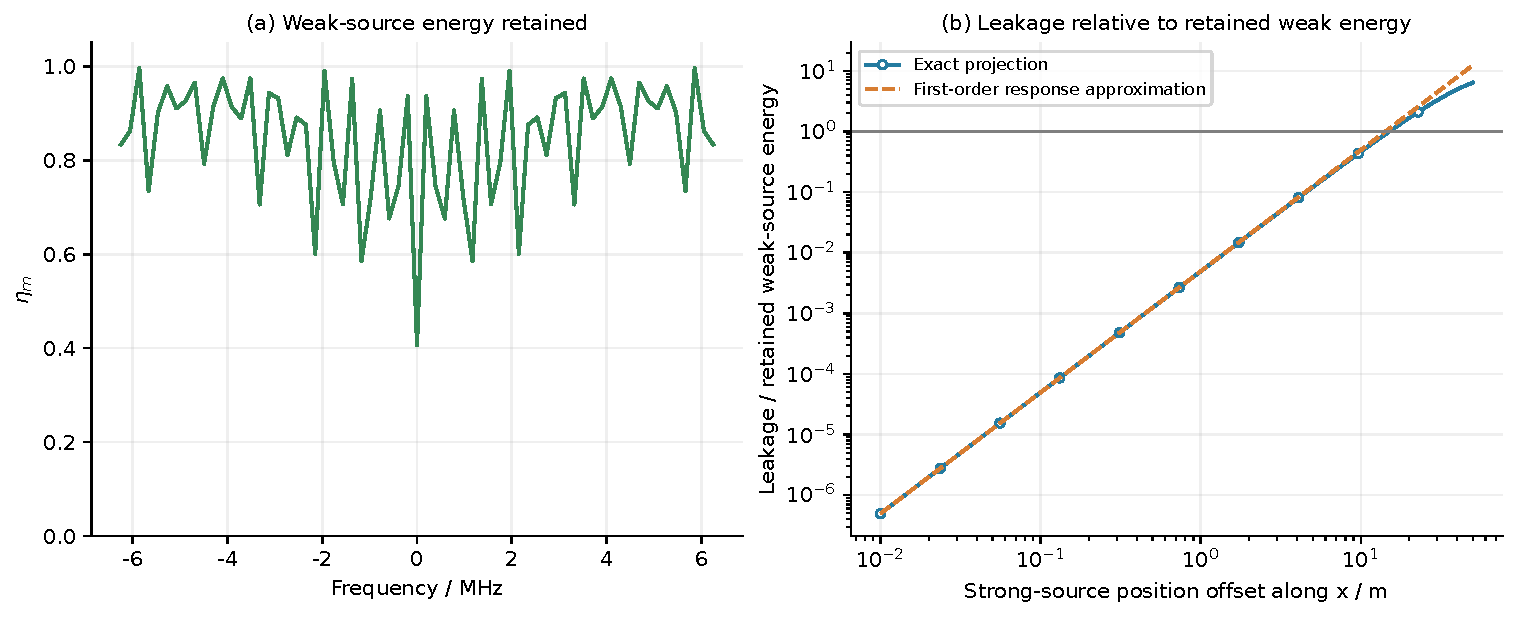
\includegraphics[width=.85\linewidth]{figures/fig_3_4.pdf}
\caption{Numerical illustration of projection loss and leakage.}\label{fig:3.4}
\begin{minipage}{\linewidth}\small
The frequency-domain parameters are specified in this subsection. (a) Retained weak-source energy fraction $\eta_m$ at each frequency. (b) Strong-source leakage divided by the weak-source energy retained under exact projection, for strong-source offsets of 0.01 to 50 m along $x$. The first-order response approximation in (\ref{eq:2.16}) is also shown. The energy ratio grows approximately quadratically for small offsets.
\end{minipage}
\end{figure}

% Source block 151
For small offsets, the leakage agrees with the quadratic energy approximation in (\ref{eq:2.16}). This explains why a strong-source error below the success threshold may still affect weak-source search, but it does not supply a practical stopping rule for strong-source refinement. The conditional-score results in Section~\ref{sec:3.5} are consistent with this error-propagation mechanism.

% Source block 152
\subsection{Success rates, processing time, and error distributions}\label{sec:3.8}

% Source block 153
\begin{figure}[!htbp]
\centering
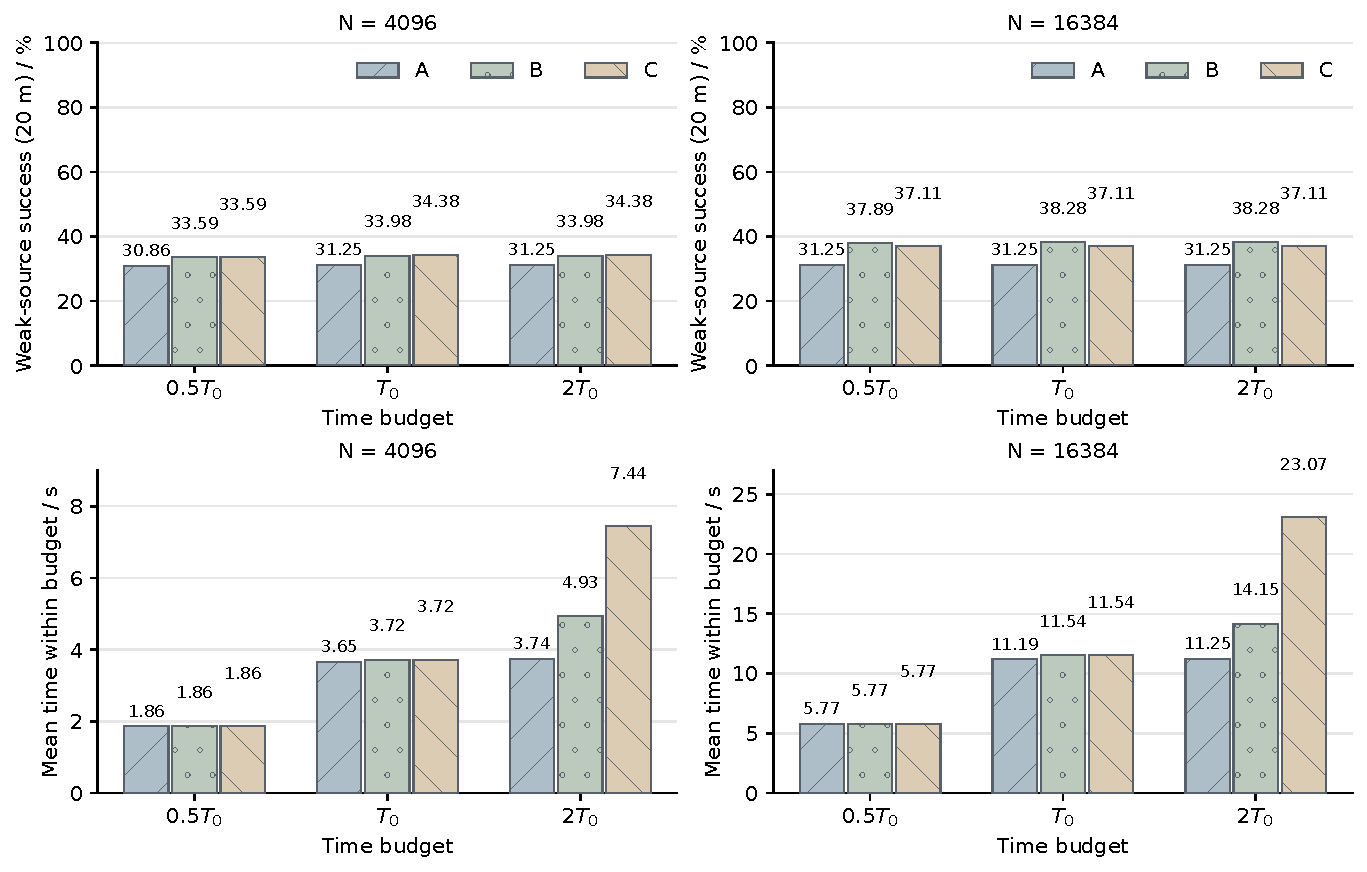
\includegraphics[width=.94\linewidth]{figures/fig_3_5.pdf}
\caption{Weak-source success and online time at three budgets.}\label{fig:3.5}
\begin{minipage}{\linewidth}\small
Each method and record length has 256 mixed conditions. The abscissa gives budgets $0.5T_0,T_0,2T_0$. The upper panels show weak-source success within 20 m. The lower panels report mean online processing time capped at each budget: actual time for runs that finish early and the deadline otherwise. The last completed output before the deadline is evaluated. Table~\ref{tab:3.8} separately reports measured time over the entire run window.
\end{minipage}
\end{figure}

% Source block 156
\begin{table}[H]
\centering
\caption{Mean measured processing time with a run limit of $2T_0$.}\label{tab:3.8}
\small
\setlength{\tabcolsep}{4pt}
\renewcommand{\arraystretch}{1.2}
\begin{tabularx}{\linewidth}{Y{1}Y{1}Y{1}Y{1}Y{1}}
\toprule
\textbf{Samples} & \textbf{A / s} & \textbf{B / s} & \textbf{C / s} & \textbf{C/B} \\
\midrule
4096 & 3.739 & 4.933 & 7.446 & $\approx1.51$ \\
16384 & 11.248 & 14.154 & 23.078 & $\approx1.63$ \\
\bottomrule
\end{tabularx}
\end{table}

% Source block 158
C exhausts the $2T_0$ window in 507 of 512 mixed tasks. Its additional time relative to B yields no success-rate advantage. Weak-source success changes little across the three budgets for each method, indicating that running the same search longer does not adequately improve candidate coverage under these settings.

% Source block 159
\begin{figure}[!htbp]
\centering
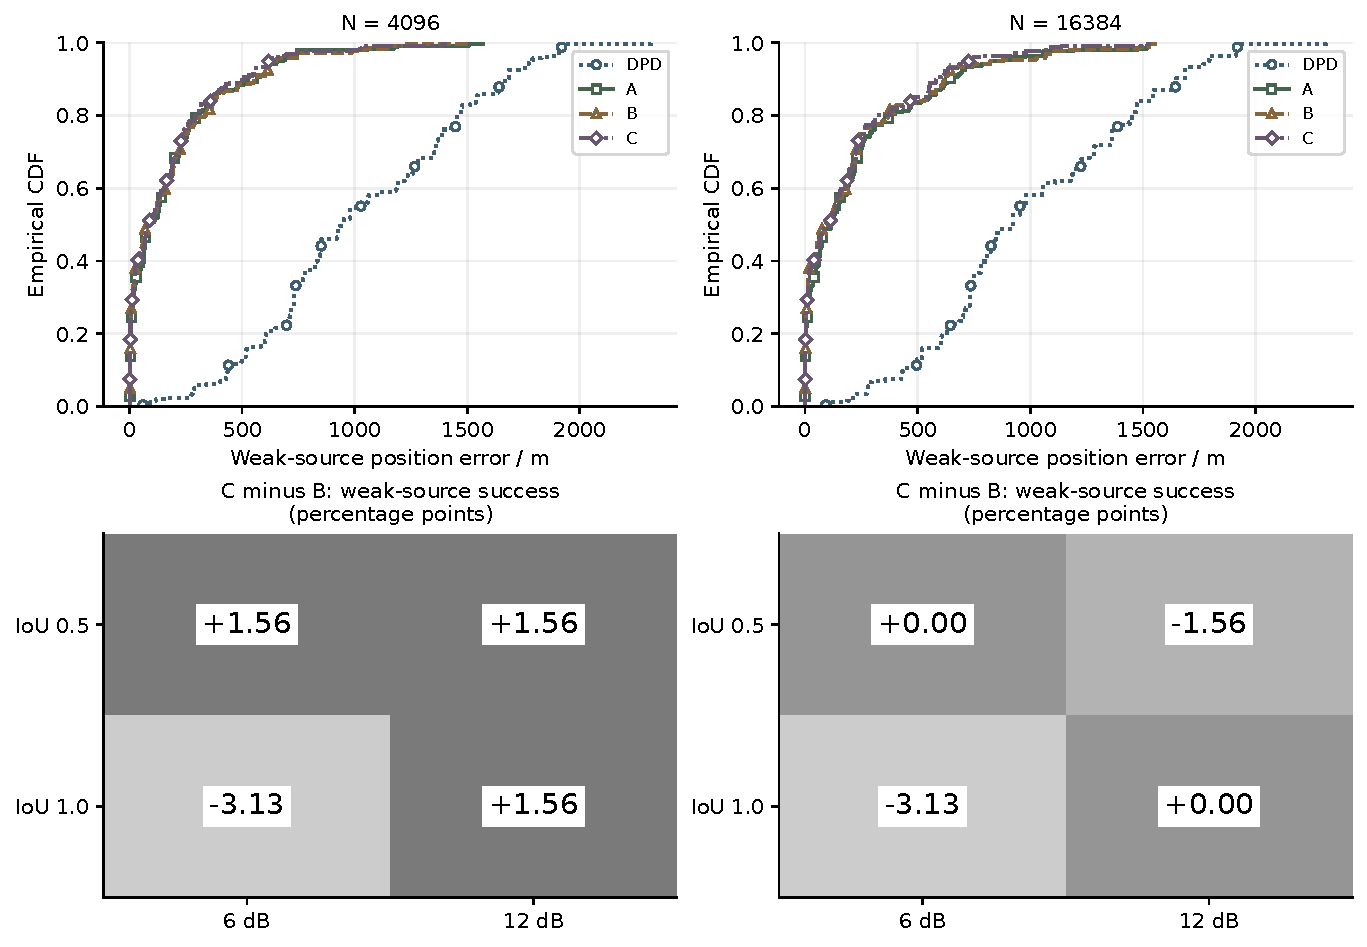
\includegraphics[width=.94\linewidth]{figures/fig_3_6.pdf}
\caption{Untruncated errors and performance by condition.}\label{fig:3.6}
\begin{minipage}{\linewidth}\small
Upper panels: weak-source error CDFs under minimum-squared-distance assignment, with 256 records per curve. Lower panels: the difference in 20 m weak-source success rate between C and B, in percentage points, for each length, overlap, and power difference, with 64 records per cell. The error axis includes all observed values.
\end{minipage}
\end{figure}

% Source block 162
The error distributions in Figure~\ref{fig:3.6} have long tails, and the success-rate difference between C and B varies with the condition. Lower RMSE does not necessarily imply higher success probability. Search strategies therefore need to be assessed using success rate, untruncated error, and processing time together.

% Source block 163
\FloatBarrier
\subsection{Benefits and cost of more extensive search}\label{sec:3.9}

Following the diagnosis in Section~\ref{sec:3.6}, method D is evaluated on six new layouts with its 5 m grid, top 5 candidates, and update rounds fixed. Each layout has two record lengths, two spectral overlaps, and two power differences, giving $6\times2\times2\times2=48$ conditions, each with one waveform/noise realization. Complete methods B and D process the same observations and execute their prescribed procedures. They do not use the deadline outputs from the first experiment.

\begin{table}[H]
\centering
\caption{Complete-solver results on six new layouts, with a 20 m success radius.}\label{tab:3.9}
\small
\setlength{\tabcolsep}{4pt}
\renewcommand{\arraystretch}{1.2}
\begin{tabularx}{\linewidth}{Y{0.80}Y{0.95}Y{0.95}Y{1.05}Y{1.05}Y{1.05}Y{1.05}Y{1.10}}
\toprule
Method & \shortstack[l]{Weak\\successes} & \shortstack[l]{Both\\successful} & \shortstack[l]{Strong\\successes} & \shortstack[l]{GOSPA\\ / m} & \shortstack[l]{RMSE\\ / m} & \shortstack[l]{P95\\ / m} & \shortstack[l]{Mean time\\ / s} \\
\midrule
B & 8/48 & 8/48 & 48/48 & 69.16 & 128.56 & 343.98 & 8.04 \\
D & 40/48 & 40/48 & 48/48 & 18.37 & 64.28 & 121.40 & 31.10 \\
\bottomrule
\end{tabularx}
\end{table}

D recovers 32 weak-source failures of B and retains all 8 of its successes. Weak-source success rises from 16.67\% to 83.33\%, and overall RMSE falls from 128.56 m to 64.28 m, while mean total processing time increases by a factor of 3.87. This result measures the combined effect of supplementary global search and joint updates; their separate contributions have not been quantified.

\begin{figure}[!htbp]
\centering
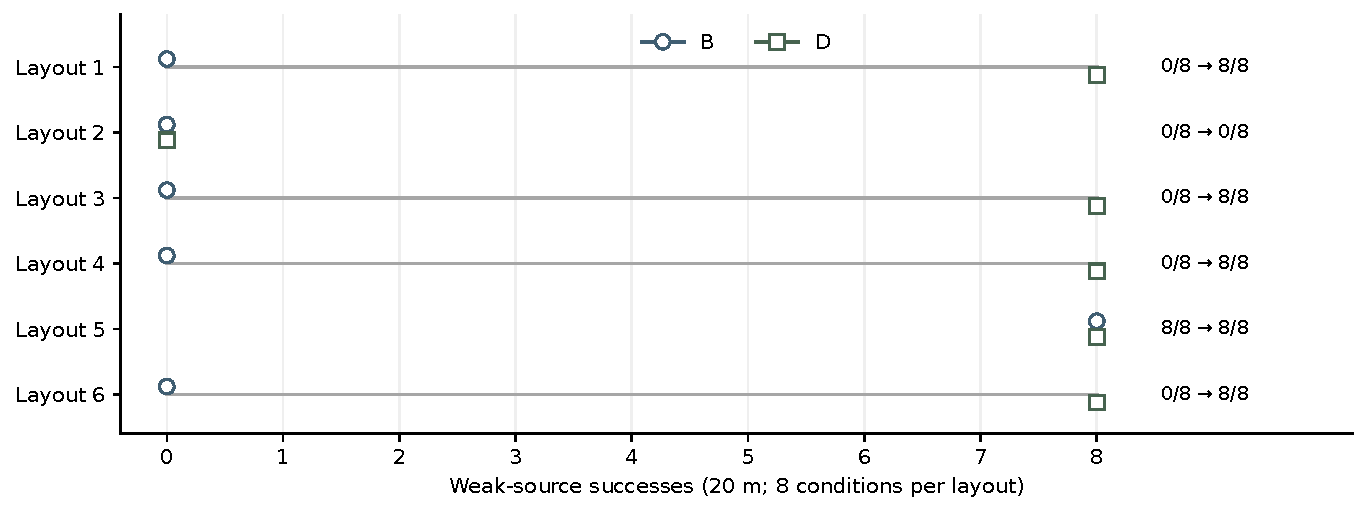
\includegraphics[width=.95\linewidth]{figures/fig_3_7.pdf}
\caption{Weak-source success counts for B and D in the six new layouts.}\label{fig:3.7}
\begin{minipage}{\linewidth}\small
Each layout contains 8 conditions, with a 20 m success radius. Circles denote B and squares denote D. Coincident markers are offset slightly in the vertical direction; horizontal coordinates remain the actual success counts. Layout labels apply only to this comparison.
\end{minipage}
\end{figure}

\begin{figure}[!htbp]
\centering
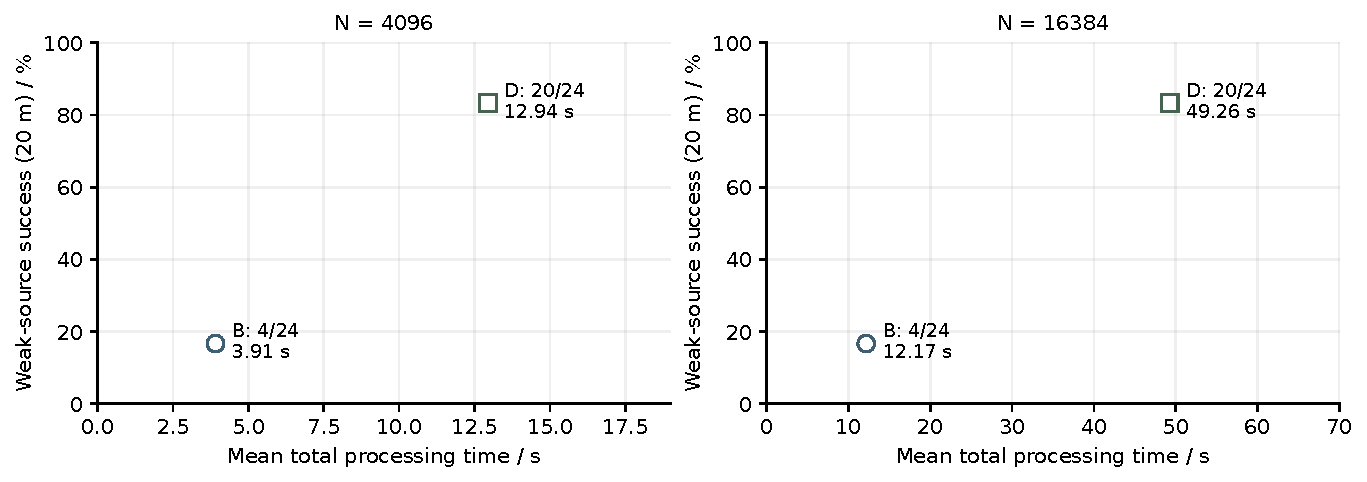
\includegraphics[width=.95\linewidth]{figures/fig_3_8.pdf}
\caption{Success rate and total processing time for the two record lengths.}\label{fig:3.8}
\begin{minipage}{\linewidth}\small
There are 24 conditions per length. Mean times for B and D are 3.91 s and 12.94 s at 4096 samples, and 12.17 s and 49.26 s at 16384 samples. D includes the complete B procedure and subsequent search, without deadline truncation.
\end{minipage}
\end{figure}

D succeeds on 20 of 24 weak-source records at each length. The remaining 8 failures all occur in layout 2, with weak-source errors from 83.72 to 290.93 m. This layout fails at both lengths, overlaps, and power differences. The concentration of failures suggests a dependence on geometry, but these results do not separate finer candidate omissions, incorrect local optima, and position coupling. This sample differs from the preceding 32-layout set; success rates and times are interpreted separately.

\subsection{Regional subdivision on fixed diagnostic records}\label{sec:3.10}

To test whether (\ref{eq:cell-upper}) can reduce search effort, four single-update weak-source searches are compared on the same 24 diagnostic records as in Section~\ref{sec:3.6}: a uniform 5 m grid; a 10 m grid shifted by 5 m along each coordinate; score-prioritized subdivision; and upper-bound-prioritized subdivision. All strategies fix the original strong-source estimate, retain the top 5 candidates, and use the same continuous refinement. An output is retained only if its score is no lower than that of the initial estimate. The 5 m scan here updates only the weak position once, unlike the sequential global searches and joint updates of complete method D.

Both subdivision strategies start from a 50 m grid with initial cell half-width 25 m. They subdivide at most 32 cells per step, evaluate at most 16384 grid points, and use a minimum half-width of 1.5625 m. Score-prioritized subdivision ranks cells by center score. Upper-bound-prioritized subdivision ranks them by $U(\mathcal C)$ and prunes a cell when its bound is below the best score found. Numerical checks cover two record lengths, zero to two fixed sources, and four cell scales, giving 24 configurations. No sampled score exceeds its cell bound. These checks assess numerical consistency, not localization performance.

\begin{table}[H]
\centering
\caption{Single weak-source updates with the estimated strong position fixed.}\label{tab:region-search}
\small
\setlength{\tabcolsep}{4pt}
\renewcommand{\arraystretch}{1.2}
\begin{tabularx}{\linewidth}{Y{1.25}Y{0.95}Y{0.95}Y{1.15}Y{1.0}Y{0.7}}
\toprule
Strategy & \shortstack[l]{Historical\\failures\\recovered} & \shortstack[l]{Historical\\controls\\successful} & \shortstack[l]{Mean grid\\evaluations} & \shortstack[l]{Mean update\\time / s} & \shortstack[l]{Cells\\pruned} \\
\midrule
Uniform 5 m grid & 15/16 & 8/8 & 160689.5 & 11.2231 & --- \\
Shifted 10 m grid & 14/16 & 8/8 & 39971.2 & 2.8870 & --- \\
Score-prioritized subdivision & 2/16 & 6/8 & 16384 & 1.2901 & --- \\
Bound-prioritized subdivision & 9/16 & 6/8 & 16384 & 1.5700 & 0 \\
\bottomrule
\end{tabularx}
\par\smallskip
\begin{minipage}{\linewidth}\small
Success means a weak-source error no greater than 20 m. Times and grid counts are averaged over all 24 records. Time includes candidate refinement but excludes the preceding strong-source estimation; grid counts exclude function evaluations during continuous optimization. Only the bound-prioritized strategy performs pruning, and its pruned-cell count is zero in every record.
\end{minipage}
\end{table}

At the same limit of 16384 grid evaluations, bound-prioritized subdivision recovers 9 of 16 historical failures, compared with 2 for score-prioritized subdivision. The bound thus improves cell ordering. Both strategies exhaust the evaluation limit, however, and the bound-prioritized strategy eliminates no cells. Its mean update time is approximately 14.0\% of the 5 m scan time, but it recovers 6 fewer failures, so recovery is not comparable. The current bound satisfies the adopted response-model constraints but is too loose to provide useful pruning.

The shifted 10 m grid recovers 14 of 16 historical failures using approximately 25.7\% of the 5 m scan time, matching the recovery count of the ordinary 10 m scan in Section~\ref{sec:3.6}. In the narrow-peak case where the two grids differ, the 5 m error is 0.805 m and the shifted 10 m error is 48.54 m. Shifting samples changes candidate positions, but these results do not show that it can reliably replace a finer grid. Both subdivision strategies succeed on 6 of the 8 historical controls, retaining all 6 original successes at 20 m. The 5 m and shifted 10 m scans also bring the other 2 controls within 20 m.

These results concern a single weak-source update with the strong estimate fixed, on purposively selected historical failures and controls. The recovery fractions are not population success rates, and the update times do not establish a speedup for the complete localization algorithm.

\subsection{Findings}\label{sec:3.11}

% Source block 164
In the 32-layout comparison, sequential projection and joint updates raise weak-source success within 20 m to 31\% to 36\%, still below the isolated-source rates of 91\% to 95\%. Conditional scores reveal better positions that the solver misses in most failures. Strong-source position errors also affect weak-source scores in some records.

% Source block 165
Response-variation ranking in C shows no consistent benefit over B. Supplementary 5 m global search in D increases weak-source successes from 8 of 48 to 40 of 48 in six new layouts, at 3.87 times the mean total processing time. On the fixed diagnostic sample, the regional bound improves subdivision order but produces no pruning and recovers fewer failures than the dense grid. Search design must reduce unproductive evaluations while preserving narrow-peak candidates. Longer runs or a different ranking alone have not resolved this tradeoff.

% Source block 166
All conditions in one layout still fail after the complete dense-search procedure. The single-update comparisons with a fixed strong estimate do not explain those remaining failures. Candidate omissions and position coupling must be separated to determine when both source positions should change together.

% Source block 168
\section{Discussion of the known-gain experiments}\label{sec:4}

The following discussion retains the search and joint-update questions raised by the known-relative-gain experiments in Appendix~\ref{sec:3}. Whether the same behavior occurs with unknown gains remains to be tested in the main-text experiment.

% Source block 169
\subsection{Narrow-peak width and search scale}\label{sec:4.1}

% Source block 170
In Table~\ref{tab:3.7}, the grid point 4.523 m from the true position scores below a distant incorrect peak, while a local solution near the truth has error 0.803 m. Equation~(\ref{eq:2.17}) describes second-order behavior near a peak, but neither its location nor its curvature is known before the search. It therefore does not directly determine grid spacing.

% Source block 171
Equation~(\ref{eq:cell-upper}) provides a regional score bound from response perturbations, yet it yields no pruning in the present comparison. When the projected-response norm is small or phase changes substantially across a cell, the directional constraint can reduce to the residual-energy bound. The remaining question is how to use center scores, response derivatives, and residuals to tighten the bound at acceptable cost. Equivalent Fisher information describes local statistical accuracy, whereas the score Hessian describes peak shape for one observation. Conditions under which either can guide search scale need to be established.

% Source block 172
\subsection{Candidate selection and computational allocation}\label{sec:4.2}

% Source block 173
In 292 of 327 weak-source failures, the true weak position already scores higher under the original strong estimate. D recovers many failures on new layouts, but its mean time is 3.87 times that of B. On the fixed records, bound-prioritized subdivision also recovers fewer failures than the simple shifted grid. A more elaborate cell rule does not necessarily preserve more useful candidates for a given computational cost. When a cell center has a low score, what observed information justifies further subdivision? A few additional samples, residual correlations, or curvature estimates may help reduce uniform global refinement, but their cost and recovery must be assessed together.

% Source block 174
Multiple delay hypotheses are another possible source of position candidates. Relative to receiver 1, position determines the delay difference
% Source block 175
\begin{equation}\label{eq:4.1}
\Delta\tau_{\ell1}(\mathbf{p}) = \frac{\|\mathbf{p}-\mathbf{r}_\ell\|-\|\mathbf{p}-\mathbf{r}_1\|}{c}.
\end{equation}

% Source block 176
Several correlation peaks could be retained, geometric consistency used to generate position candidates, and the joint residual used to select among them\cite{ref01,ref02,ref03}. The unresolved choices are whether to estimate delays from the raw mixture or the residual after strong-source projection, and when to impose cross-receiver constraints so that incorrect combinations are reduced without discarding weak-source hypotheses too early. Correlation computation, hypothesis combinations, and signal-domain validation must all be included in processing time.

% Source block 177
In the same selected cases, increasing the retained candidate count from 5 to 32 on a 10 m grid gives no additional recovery, whereas a 5 m grid with 5 candidates recovers more records. Candidate count and sampling density therefore require separate treatment. New selection rules should retain uniform and shifted grids as references, compare recovery and cost under the same continuous-refinement configuration, and account for total time in the complete solver.

% Source block 178
\Needspace{.23\textheight}
\subsection{Strong-source accuracy and joint position updates}\label{sec:4.3}

% Source block 179
In the conditional-score analysis, substituting the true strong position restores a score advantage at the true weak position in 22 records, including one whose original strong-source error is below 20 m. Equation~(\ref{eq:2.16}) approximates leakage for small errors, but the true error is unavailable during estimation, and the success threshold cannot determine when refinement should stop. The remaining failures of D occur in one layout, raising the question of whether sequential updates are constrained by coupled local solutions.

% Source block 180
Can local curvature, response derivatives, and residuals estimate the benefit of refining the strong position versus searching again for the weak source? Alternating updates change one position at a time and may repeatedly return to the same local solution. When to retain multiple strong-position hypotheses or update all four position coordinates jointly remains unresolved. In a four-receiver system, expanding the suppression subspace also reduces the retained dimension\cite{ref07}. These alternatives therefore need to be compared in terms of strong-source leakage, loss of weak-source information, and additional computation.

% Source block 182
\clearpage
\end{document}
